% ============================================================
%  DS200.Q21 — Tái triển khai và Cải tiến ViHateT5
%  cho Phát hiện Ngôn từ Thù ghét Tiếng Việt
%  Beamer Presentation — Nhóm 02 (Tiếng Việt)
% ============================================================
\documentclass[11pt, aspectratio=169]{beamer}
\usetheme{Frankfurt}
\usefonttheme{serif}

% --- Vietnamese ---
\usepackage{fontspec}
\setmainfont{texgyretermes}[
    Extension      = .otf,
    UprightFont    = *-regular,
    BoldFont       = *-bold,
    ItalicFont     = *-italic,
    BoldItalicFont = *-bolditalic
]
\usepackage{polyglossia}
\setdefaultlanguage{vietnamese}

% --- Packages ---
\usepackage{tikz}
\usetikzlibrary{arrows.meta, positioning, shapes.geometric, fit, calc}
\usepackage{amsmath,amssymb,graphicx,booktabs}
\usepackage{hyperref}
\usepackage[table]{xcolor}
\hypersetup{colorlinks=true,urlcolor=blue}
\usepackage{listings}
\usepackage{multicol}
\usepackage{caption}
\usepackage{multirow}
\usepackage{array}
\usepackage{colortbl}

\setbeamerfont{caption}{size=\tiny}
\setbeamertemplate{caption}[numbered]

% --- Main colors ---
\definecolor{uitblue}{RGB}{0,70,140}
\definecolor{uitdarkblue}{RGB}{0,50,100}
\definecolor{uitlightblue}{RGB}{220,235,250}
\definecolor{successgreen}{RGB}{40,140,40}
\definecolor{alertorange}{RGB}{210,105,30}

\setbeamercolor{structure}{fg=uitblue}
\setbeamercolor{frametitle}{fg=white,bg=uitblue}
\setbeamercolor{title}{fg=white, bg=uitblue}
\setbeamercolor{block title}{bg=uitblue!80,fg=white}
\setbeamercolor{block body}{bg=blue!5,fg=black}
\setbeamercolor{section in head/foot}{fg=white, bg=uitblue}
\setbeamercolor{subsection in head/foot}{fg=white, bg=uitdarkblue}
\setbeamercolor{item}{fg=uitblue}

% Green block
\setbeamercolor{block title example}{fg=white, bg=successgreen}
\setbeamercolor{block body example}{bg=green!5!white}

% Orange block
\setbeamercolor{block title alerted}{fg=white, bg=alertorange}
\setbeamercolor{block body alerted}{bg=orange!5!white}

% Bullet styling
\setbeamertemplate{itemize item}{\color{uitblue}\small$\blacktriangleright$}
\setbeamertemplate{itemize subitem}{\color{uitblue!70}\footnotesize$\triangleright$}
\setbeamertemplate{enumerate item}{\color{uitblue}\insertenumlabel.}

% --- Figure path ---
\graphicspath{{../results/images/}{images/}{figures/}}

% --- Footer ---
\setbeamertemplate{footline}{
  \leavevmode%
  \hbox{%
    \begin{beamercolorbox}[wd=.33\paperwidth,ht=2.2ex,dp=1ex,center]{author in head/foot}%
      GVHD: TS. Hà Minh Tân
    \end{beamercolorbox}%
    \begin{beamercolorbox}[wd=.34\paperwidth,ht=2.2ex,dp=1ex,center]{title in head/foot}%
      DS200.Q21 -- Phân tích Dữ liệu Lớn
    \end{beamercolorbox}%
    \begin{beamercolorbox}[wd=.33\paperwidth,ht=2.2ex,dp=1ex,center]{date in head/foot}%
      \today \hspace{1em} \insertframenumber{} / \inserttotalframenumber
    \end{beamercolorbox}%
  }%
  \vskip0pt%
}
\setbeamertemplate{navigation symbols}{}

% --- Show outline before each section ---
\AtBeginSection[]{
  \begin{frame}{Mục lục}
    \tableofcontents[currentsection]
  \end{frame}
}

% --- Title ---
\title[ViHateT5]{\textbf{Tái triển khai và Cải tiến ViHateT5 \\ cho Phát hiện Ngôn từ Thù ghét Tiếng Việt} \\ \textbf{(Reimplementation and Improvement of ViHateT5 \\ for Vietnamese Hate Speech Detection)}}

\author[DS200.Q21]{DS200.Q21 -- Phân tích Dữ liệu Lớn -- Nhóm 02 \\[0.3em]
Nguyễn Công Phát \and Trương Hoàng Thành An \and Vũ Việt Cương \\
23521143 \and 23520032 \and 23520213}
\institute[UIT]{Trường Đại học Công nghệ Thông tin -- ĐHQG TP.HCM}
\date{GVHD: TS. Hà Minh Tân}

% ============================================================
\begin{document}

% ---------- Title ----------
\begin{frame}[plain]
  \titlepage
\end{frame}

% ---------- Outline ----------
\begin{frame}{Mục lục}
  \tableofcontents
\end{frame}

% ============================================================
\section{Giới thiệu tổng quan}
% ============================================================

\begin{frame}[fragile, shrink=10]{1.1. Bối cảnh và Vấn đề}
\begin{columns}[T]
  \column{0.55\textwidth}
  \begin{block}{Ngôn từ thù ghét trên mạng xã hội}
    \begin{itemize}
      \item Sự bùng nổ nội dung tiếng Việt trên mạng xã hội
      \item Ngôn từ thù ghét, xúc phạm lan truyền nhanh chóng
      \item Kiểm duyệt thủ công \textbf{không khả thi} ở quy mô lớn
      \item Hệ thống phát hiện tự động là cấp thiết
    \end{itemize}
  \end{block}

  \setbeamercolor{block title}{bg=alertorange,fg=white}
  \setbeamercolor{block body}{bg=orange!5,fg=black}
  \begin{block}{Thách thức}
    \begin{itemize}
      \item Nhiều \textbf{bài toán} HSD khác nhau (phân loại, xác định vùng)
      \item Dữ liệu gán nhãn cho tiếng Việt còn hạn chế
      \item Mất cân bằng nhãn trong các bộ dữ liệu hiện có
      \item Mỗi bài toán cần một mô hình riêng $\Rightarrow$ phân mảnh hệ thống
    \end{itemize}
  \end{block}

  \column{0.42\textwidth}
  \setbeamercolor{block title}{bg=successgreen,fg=white}
  \setbeamercolor{block body}{bg=green!5,fg=black}
  \begin{block}{Bộ dữ liệu hiện có}
    \begin{itemize}
      \item \textbf{ViHSD}: 33K bình luận (3 nhãn)
      \item \textbf{ViCTSD}: 10K bình luận (2 nhãn)
      \item \textbf{ViHOS}: 11K bình luận (hate spans)
      \item \textbf{VOZ-HSD}: 10.8M+ bình luận thô
    \end{itemize}
  \end{block}

  \vspace{0.3cm}
  \setbeamercolor{block title}{bg=uitblue!80,fg=white}
  \setbeamercolor{block body}{bg=blue!5,fg=black}
  \begin{block}{Mục tiêu}
    Xây dựng mô hình \textbf{thống nhất} cho phát hiện ngôn từ thù ghét tiếng Việt trên nhiều bài toán và bộ dữ liệu.
  \end{block}
\end{columns}
\end{frame}

% ----------------------------------------------------------
\begin{frame}{1.2. Lý do thực hiện}
\scriptsize

\setbeamercolor{block title}{bg=uitblue!80,fg=white}
\setbeamercolor{block body}{bg=blue!5,fg=black}
\begin{block}{Bối cảnh}
  \begin{itemize}
    \item Các mô hình hiện tại chủ yếu train trên Wikipedia, còn HSD xảy ra trên mạng xã hội với teencode, từ lóng
    \item Trước đây, mỗi bài toán (Toxic, Hate, Spans) cần một model riêng $\Rightarrow$ phức tạp hệ thống
    \item Cần kiểm chứng khả năng ``hiểu'' ngôn ngữ của kiến trúc T5 so với Encoder-only (BERT)
  \end{itemize}
\end{block}

\vspace{0.3cm}
\centering
\renewcommand{\arraystretch}{1.15}
\rowcolors{2}{blue!3!white}{white}
\resizebox{0.95\textwidth}{!}{%
\begin{tabular}{|p{3cm}|p{5.5cm}|p{4.5cm}|}
\hline
\rowcolor{uitblue!90!black}
\textcolor{white}{\textbf{Tiếp cận}} &
\textcolor{white}{\textbf{Mô tả}} &
\textcolor{white}{\textbf{Hạn chế}} \\
\hline
\textbf{Class-specific} & Một model cho một task duy nhất & Không mở rộng được \\
\hline
\textbf{Multi-model} & Nhiều model BERT cho nhiều task & Phân mảnh, tốn tài nguyên \\
\hline
\textbf{Unified T5 (ViHateT5)} & Một model cho tất cả task & \textbf{Chưa được kiểm chứng độc lập} \\
\hline
\end{tabular}
}

\vspace{0.3cm}
\setbeamercolor{block title}{bg=successgreen,fg=white}
\setbeamercolor{block body}{bg=green!5,fg=black}
\begin{block}{Mục tiêu của nhóm}
  Tái lập lại mô hình để kiểm chứng kết quả, đồng thời \textbf{đề xuất cải tiến} data-centric vượt bài báo gốc.
\end{block}
\end{frame}

% ----------------------------------------------------------
\begin{frame}[shrink=5]{1.3. Bài báo tham khảo}

\setbeamercolor{block title}{bg=uitblue!80,fg=white}
\setbeamercolor{block body}{bg=blue!5,fg=black}
\begin{block}{Bài báo gốc -- ViHateT5 (ACL 2024 Findings)}
  \textbf{Luan Thanh Nguyen}, ``\textit{ViHateT5: Enhancing Hate Speech Detection in Vietnamese With a Unified Text-to-Text Transformer Model},'' Findings of ACL 2024, pp.\,5948--5961.
\end{block}
\vspace{0.2cm}

\begin{columns}[T]
  \column{0.48\textwidth}
  \begin{block}{Đóng góp chính của bài báo}
    \begin{enumerate}
      \item Mô hình \textbf{text-to-text thống nhất} cho 3 bài toán HSD tiếng Việt
      \item Bộ dữ liệu \textbf{VOZ-HSD} 10.8M+ bình luận với nhãn tự động
      \item \textbf{Continual pre-training} với Span Corruption trên dữ liệu miền
      \item Đạt SOTA trên tất cả benchmark HSD tiếng Việt
    \end{enumerate}
  \end{block}

  \column{0.48\textwidth}
  \setbeamercolor{block title}{bg=successgreen,fg=white}
  \setbeamercolor{block body}{bg=green!5,fg=black}
  \begin{block}{Đóng góp của nhóm}
    \begin{enumerate}
      \item \textbf{Tái triển khai} đầy đủ ViHateT5
      \item Pipeline \textbf{gán nhãn tự động} với ViSoBERT (10M+ mẫu, 97.5\% accuracy)
      \item Mở rộng \textbf{8 baselines BERT}
      \item \textbf{Cải tiến data-centric} vượt bài báo gốc
      \item Mô hình đăng trên HuggingFace
    \end{enumerate}
  \end{block}
\end{columns}
\end{frame}

% ----------------------------------------------------------
\begin{frame}[shrink=10]{1.3b. Công trình liên quan}

\begin{table}[h]
  \centering
  \caption{Các phương pháp HSD tiêu biểu trước ViHateT5}
  \vspace{0.2cm}
  \resizebox{0.95\textwidth}{!}{%
  \begin{tabular}{llllp{4cm}}
    \toprule
    \textbf{Mô hình} & \textbf{Năm} & \textbf{Venue} & \textbf{Tiếp cận} & \textbf{Hạn chế} \\
    \midrule
    HateBERT & 2021 & ACL Workshop & BERT pre-trained trên Reddit & Chỉ tiếng Anh, encoder-only \\
    PhoBERT & 2020 & EMNLP Findings & RoBERTa cho tiếng Việt & Formal text (Wiki+News), 1 task/model \\
    ViSoBERT & 2023 & EMNLP & BERT trên MXH Việt & Encoder-only, 1 task/model \\
    ViT5 & 2022 & COLING & T5 cho tiếng Việt (CC100) & Chưa domain-specific cho HSD \\
    mT5 & 2021 & NAACL & T5 đa ngôn ngữ (101 langs) & Không chuyên biệt tiếng Việt \\
    \midrule
    \rowcolor{uitlightblue}
    \textbf{ViHateT5} & \textbf{2024} & \textbf{ACL Findings} & \textbf{T5 + domain pre-train VOZ} & \textbf{Chưa kiểm chứng độc lập} \\
    \bottomrule
  \end{tabular}}
\end{table}

\begin{columns}[T]
  \column{0.48\textwidth}
  \setbeamercolor{block title}{bg=uitblue!80,fg=white}
  \setbeamercolor{block body}{bg=blue!5,fg=black}
  \begin{block}{Xu hướng}
    \begin{itemize}
      \item Encoder-only $\rightarrow$ Encoder-Decoder
      \item Single-task $\rightarrow$ Multi-task unified
      \item General corpus $\rightarrow$ Domain-specific data
    \end{itemize}
  \end{block}

  \column{0.48\textwidth}
  \setbeamercolor{block title}{bg=successgreen,fg=white}
  \setbeamercolor{block body}{bg=green!5,fg=black}
  \begin{block}{Gap mà ViHateT5 giải quyết}
    \begin{itemize}
      \item Unified model cho 3 tasks HSD tiếng Việt
      \item Pre-train trên 10.8M bình luận MXH thật
      \item Text-to-Text linh hoạt hơn classification head
    \end{itemize}
  \end{block}
\end{columns}
\end{frame}

% ----------------------------------------------------------
\begin{frame}[fragile, shrink=5]{1.4. Tổng quan kiến trúc ViHateT5}

\begin{center}
  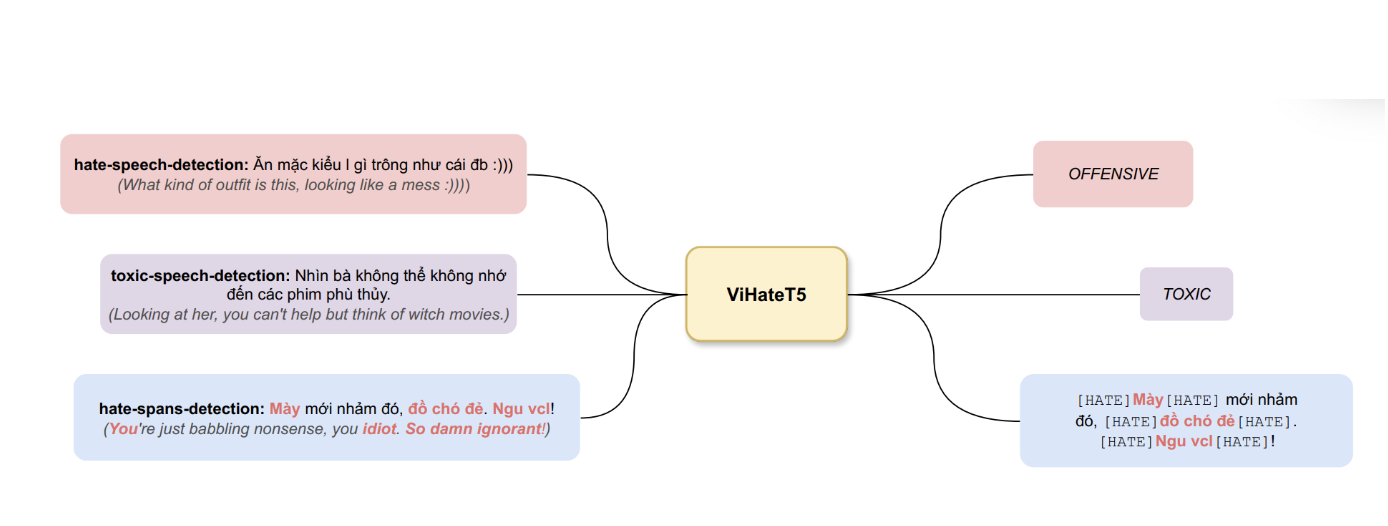
\includegraphics[width=0.88\textwidth]{Tong-quan-HSD-multitask-ViHATET5.png}
  \captionof{figure}{Kiến trúc đa nhiệm ViHateT5: một mô hình Text-to-Text xử lý 3 bài toán HSD tiếng Việt.}
\end{center}

\vspace{0.2cm}
\begin{block}{Ý tưởng cốt lõi -- Kỹ thuật Task Prefix (Tiền tố)}
  Sử dụng \textbf{Task Prefix} để hợp nhất 3 bài toán HSD khác nhau vào một mô hình Text-to-Text duy nhất, thay vì cần 3 mô hình riêng biệt.
\end{block}
\end{frame}

% ----------------------------------------------------------
\begin{frame}[fragile, shrink=10]{1.4b. Chi tiết kiến trúc T5 Encoder-Decoder}

\begin{columns}[T]
  \column{0.48\textwidth}
  \begin{block}{Kiến trúc T5 (Text-to-Text Transfer Transformer)}
    \begin{itemize}
      \item \textbf{Encoder}: Xử lý input text, tạo contextualized representations
      \item \textbf{Decoder}: Sinh output text (nhãn, span marking) theo dạng autoregressive
      \item \textbf{Attention}: Multi-head self-attention + cross-attention
      \item \textbf{Params}: ViT5-base $\approx$ 220M parameters
    \end{itemize}
  \end{block}

  \vspace{0.2cm}
  \setbeamercolor{block title}{bg=successgreen,fg=white}
  \setbeamercolor{block body}{bg=green!5,fg=black}
  \begin{block}{Ưu điểm của Text-to-Text}
    \begin{itemize}
      \item Mọi NLP task $\Rightarrow$ cùng một framework
      \item Không cần task-specific head
      \item Output linh hoạt: label, text, span
    \end{itemize}
  \end{block}

  \column{0.48\textwidth}
  \setbeamercolor{block title}{bg=uitblue!80,fg=white}
  \setbeamercolor{block body}{bg=blue!5,fg=black}
  \begin{block}{So sánh kiến trúc}
    \centering
    \resizebox{\textwidth}{!}{%
    \begin{tabular}{lcc}
      \toprule
      \textbf{Đặc điểm} & \textbf{BERT} & \textbf{T5} \\
      \midrule
      Kiến trúc & Encoder-only & Enc-Dec \\
      Output & Vector $\rightarrow$ head & Text \\
      Multi-task & Cần nhiều head & Một model \\
      Flexibility & Thấp & Cao \\
      Inference & Nhanh & Chậm hơn \\
      Span detection & BIO tagging & [HATE] markup \\
      \bottomrule
    \end{tabular}}
  \end{block}

  \vspace{0.2cm}
  \setbeamercolor{block title}{bg=alertorange,fg=white}
  \setbeamercolor{block body}{bg=orange!5,fg=black}
  \begin{block}{Ví dụ Input/Output}
    \scriptsize
    \texttt{Input: hate-speech-detection: Mày ngu quá!}\\
    \texttt{Output: HATE}\\[0.2em]
    \texttt{Input: hate-spans-detection: Mày ngu quá!}\\
    \texttt{Output: [HATE]Mày[HATE] [HATE]ngu[HATE] quá!}
  \end{block}
\end{columns}
\end{frame}

% ----------------------------------------------------------
\begin{frame}[fragile, shrink=30]{1.4c. Cơ chế Task Prefix -- Chi tiết}

\begin{block}{Nguyên lý hoạt động}
  Task Prefix là chuỗi ký tự đặt trước input để ``hướng dẫn'' mô hình thực hiện bài toán cụ thể.
  Mô hình T5 học cách \textbf{routing} dựa trên prefix $\Rightarrow$ cùng một encoder nhưng decoder sinh output khác nhau.
\end{block}

\vspace{0.2cm}
\centering
\resizebox{0.92\textwidth}{!}{%
\begin{tabular}{p{2cm}p{5.5cm}p{3cm}p{3.5cm}}
  \toprule
  \textbf{Task} & \textbf{Input Format} & \textbf{Expected Output} & \textbf{Bộ dữ liệu} \\
  \midrule
  HSD & \texttt{hate-speech-detection: \{text\}} & CLEAN / OFFENSIVE / HATE & ViHSD (33,400) \\
  TSD & \texttt{toxic-speech-detection: \{text\}} & NONE / TOXIC & ViCTSD (10,000) \\
  Spans & \texttt{hate-spans-detection: \{text\}} & Text với [HATE] markers & ViHOS (11,056) \\
  \bottomrule
\end{tabular}}

\vspace{0.3cm}
\begin{columns}[T]
  \column{0.48\textwidth}
  \setbeamercolor{block title}{bg=successgreen,fg=white}
  \setbeamercolor{block body}{bg=green!5,fg=black}
  \begin{block}{Lợi ích}
    \begin{itemize}
      \item Shared knowledge giữa các tasks
      \item Regularization effect -- giảm overfitting
      \item Giảm chi phí triển khai (1 model thay 3)
    \end{itemize}
  \end{block}

  \column{0.48\textwidth}
  \setbeamercolor{block title}{bg=uitblue!80,fg=white}
  \setbeamercolor{block body}{bg=blue!5,fg=black}
  \begin{block}{Multi-task Learning}
    \begin{itemize}
      \item Huấn luyện đồng thời trên 3 datasets
      \item Proportional mixing (theo kích thước dataset)
      \item Gradient update từ tất cả tasks
    \end{itemize}
  \end{block}
\end{columns}
\end{frame}

% ----------------------------------------------------------
\begin{frame}[shrink=5]{1.4d. Pipeline tổng quan -- 3 Giai đoạn}

\begin{center}
\begin{tikzpicture}[
  node distance=0.8cm,
  stage/.style={rectangle, rounded corners=6pt, minimum width=3.8cm, minimum height=1.6cm, align=center, font=\small\bfseries, draw=none},
  arrow/.style={-{Stealth[length=8pt]}, line width=1.5pt, uitblue!70},
  label/.style={font=\scriptsize, align=center, text width=4cm}
]
  % Stage 1
  \node[stage, fill=uitblue!15, draw=uitblue!60, line width=1pt] (s1) {Stage 1\\Pre-training\\(Span Corruption)};
  % Stage 2
  \node[stage, fill=successgreen!15, draw=successgreen!60, line width=1pt, right=1.5cm of s1] (s2) {Stage 2\\Fine-tuning\\(Multi-task Seq2Seq)};
  % Stage 3
  \node[stage, fill=alertorange!15, draw=alertorange!60, line width=1pt, right=1.5cm of s2] (s3) {Stage 3\\Inference\\(Ensemble + Deploy)};

  % Arrows
  \draw[arrow] (s1) -- (s2);
  \draw[arrow] (s2) -- (s3);

  % Labels below
  \node[label, below=0.4cm of s1] {ViT5-base\\+ 10.8M VOZ comments\\lr=5e-3, epochs=10};
  \node[label, below=0.4cm of s2] {3 datasets (ViHSD,\\ViCTSD, ViHOS)\\lr=2e-4, epochs=4};
  \node[label, below=0.4cm of s3] {Dirichlet weight search\\INT8 quantization\\FastAPI + Streamlit};
\end{tikzpicture}
\end{center}

\vspace{0.3cm}
\begin{columns}[T]
  \column{0.32\textwidth}
  \setbeamercolor{block title}{bg=uitblue!80,fg=white}
  \setbeamercolor{block body}{bg=blue!5,fg=black}
  \begin{block}{\centering Input}
    \centering VietAI/vit5-base\\(223M params)
  \end{block}

  \column{0.32\textwidth}
  \setbeamercolor{block title}{bg=successgreen,fg=white}
  \setbeamercolor{block body}{bg=green!5,fg=black}
  \begin{block}{\centering Objective}
    \centering Maximize F1-macro\\trên 3 tasks
  \end{block}

  \column{0.32\textwidth}
  \setbeamercolor{block title}{bg=alertorange,fg=white}
  \setbeamercolor{block body}{bg=orange!5,fg=black}
  \begin{block}{\centering Output}
    \centering Web app phân loại\\real-time
  \end{block}
\end{columns}
\end{frame}

% ----------------------------------------------------------
\begin{frame}[fragile, shrink=8]{1.5. Mục tiêu đồ án}

\setbeamercolor{block title}{bg=uitblue!80,fg=white}
\setbeamercolor{block body}{bg=blue!5,fg=black}
\begin{block}{Yêu cầu môn học (DS200.Q21 -- Phân tích Dữ liệu Lớn)}
  \begin{enumerate}
    \item \textbf{Hiểu} các thuật toán và mô hình AI được sử dụng để phân tích dữ liệu
    \item \textbf{Thiết kế mã} và tái triển khai bài báo
    \item \textbf{Đánh giá} điểm mạnh và điểm yếu của phương pháp, đề xuất cải tiến
    \item \textbf{Đề xuất} giải pháp cải tiến, thuật toán hoặc mô hình mới
  \end{enumerate}
\end{block}

\vspace{0.3cm}
\begin{columns}[T]
  \column{0.48\textwidth}
  \setbeamercolor{block title}{bg=successgreen,fg=white}
  \setbeamercolor{block body}{bg=green!5,fg=black}
  \begin{block}{Những gì đã tái triển khai}
    \begin{itemize}
      \item T5 continual pre-training
      \item Multi-task Seq2Seq fine-tuning
      \item 8 baselines BERT (đa ngôn ngữ + đơn ngữ)
      \item Tái tạo tất cả bảng kết quả (Tables 3--6)
    \end{itemize}
  \end{block}

  \column{0.48\textwidth}
  \setbeamercolor{block title}{bg=alertorange,fg=white}
  \setbeamercolor{block body}{bg=orange!5,fg=black}
  \begin{block}{Những gì đã cải tiến}
    \begin{itemize}
      \item Pipeline gán nhãn tự động cho VOZ-HSD
      \item Data augmentation (EDA + Back-translation)
      \item Focal Loss cho mất cân bằng lớp
      \item Ensemble nhiều mô hình
      \item Tất cả mô hình đăng trên HuggingFace
    \end{itemize}
  \end{block}
\end{columns}
\end{frame}

% ============================================================
\section{Phương pháp thực hiện}
% ============================================================

\begin{frame}[fragile, shrink=5]{2.1. Tổng quan phương pháp}

\begin{itemize}
  \item \textbf{Thu thập dữ liệu}: Thu thập 10.8 triệu bình luận từ diễn đàn VOZ để khai thác ngôn ngữ đời thực và các biểu cảm thù ghét.
  \item \textbf{Kiểm chứng và tiền xử lý}: Loại bỏ nhiễu và sử dụng mô hình ViSoBERT để gán nhãn tự động cho toàn bộ dữ liệu thô.
  \item \textbf{Huấn luyện mô hình}: Thực hiện tiền huấn luyện trên miền dữ liệu VOZ-HSD và tinh chỉnh đa nhiệm bằng kỹ thuật Task Prefix.
\end{itemize}

\vspace{0.3cm}
\begin{center}
  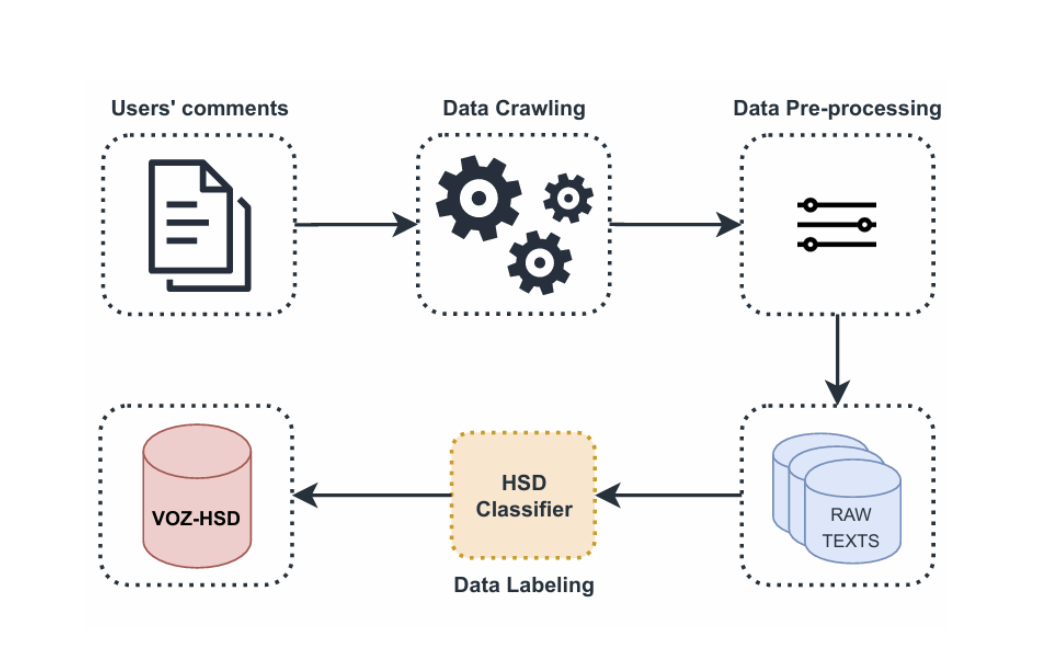
\includegraphics[width=0.75\textwidth]{So-do-quy-trinh-gan-nhan-du-lieu-VOZ-HSD.png}
  \captionof{figure}{Sơ đồ quy trình thu thập và gán nhãn dữ liệu VOZ-HSD.}
\end{center}
\end{frame}

% ----------------------------------------------------------
\begin{frame}[fragile, shrink=20]{2.2. Bước 1 -- Thu thập dữ liệu}

\begin{block}{Nguồn dữ liệu}
  \textbf{Diễn đàn VOZ} -- nền tảng mạng xã hội có tính tự do ngôn luận cao nhất Việt Nam.\\
  Phương pháp: Sử dụng công cụ \texttt{BeautifulSoup4} thu thập \textbf{10,747,733 bình luận} ($\approx$ 1.7GB).
\end{block}

\vspace{0.2cm}
\begin{columns}[T]
  \column{0.48\textwidth}
  \begin{block}{3 bộ dữ liệu downstream}
    \begin{itemize}
      \item \textbf{ViHSD}: 33,400 bình luận (Facebook, YouTube).\\
        Phân loại 3 nhãn: CLEAN / OFFENSIVE / HATE.
      \item \textbf{ViCTSD}: 10,000 mẫu (báo chí, mạng xã hội).\\
        Phát hiện tính độc hại: NONE / TOXIC.
      \item \textbf{ViHOS}: 11,056 bình luận ($>$26,000 cụm từ độc hại).\\
        Xác định vị trí thù ghét ở cấp độ âm tiết.
    \end{itemize}
  \end{block}

  \column{0.48\textwidth}
  \setbeamercolor{block title}{bg=uitblue!80,fg=white}
  \setbeamercolor{block body}{bg=blue!5,fg=black}
  \begin{block}{Mục đích}
    Sử dụng 3 bộ dataset này để so sánh hiệu năng của VIHATET5 với các mô hình đã có từ trước (baselines BERT).
  \end{block}

  \vspace{0.3cm}
  \setbeamercolor{block title}{bg=alertorange,fg=white}
  \setbeamercolor{block body}{bg=orange!5,fg=black}
  \begin{block}{Lưu ý}
    Do VOZ tăng cường bảo mật, nhóm sử dụng trực tiếp dữ liệu tác giả đã crawl sẵn để đảm bảo tái lập đúng thực nghiệm.
  \end{block}
\end{columns}
\end{frame}

% ----------------------------------------------------------
\begin{frame}[fragile, shrink=10]{2.2b. Thống kê chi tiết dữ liệu VOZ}

\begin{table}[h]
  \centering
  \caption{Phân bổ bình luận theo chủ đề trên diễn đàn VOZ}
  \vspace{0.2cm}
  \resizebox{0.88\textwidth}{!}{%
  \begin{tabular}{clrrr}
    \toprule
    \textbf{STT} & \textbf{Chủ đề (Parent Thread)} & \textbf{Số Thread} & \textbf{Số Bình luận} & \textbf{Dung lượng} \\
    \midrule
    1 & Random conversation & 142,387 & 6,104,792 & 945MB \\
    2 & News & 76,107 & 2,030,315 & 304MB \\
    3 & Sports & 10,121 & 1,154,658 & 144MB \\
    4 & Cars & 12,348 & 552,717 & 96MB \\
    5 & Movies -- Music -- Books & 6,467 & 329,601 & 52MB \\
    6 & Bikes & 5,093 & 258,728 & 41MB \\
    7 & Fashion & 1,845 & 137,548 & 19MB \\
    8 & Food -- Travel & 3,492 & 136,649 & 19MB \\
    9 & Other hobbies & 690 & 42,737 & 6MB \\
    \midrule
    & \textbf{Tổng cộng} & \textbf{258,550} & \textbf{10,747,745} & \textbf{1.66GB} \\
    \bottomrule
  \end{tabular}}
\end{table}

\begin{block}{Đặc điểm dữ liệu VOZ}
  \begin{itemize}
    \item Ngôn ngữ đời thường: teencode, từ lóng, viết tắt, emoji, meme
    \item \textbf{Random conversation} chiếm 56.8\% -- nơi tập trung ngôn từ thù ghét nhiều nhất
    \item Dữ liệu đa dạng chủ đề giúp mô hình tổng quát hóa tốt hơn
  \end{itemize}
\end{block}
\end{frame}

% ----------------------------------------------------------
\begin{frame}[fragile, shrink=10]{2.2c. Chi tiết 3 bộ dữ liệu Downstream}

\begin{columns}[T]
  \column{0.32\textwidth}
  \setbeamercolor{block title}{bg=uitblue!80,fg=white}
  \setbeamercolor{block body}{bg=blue!5,fg=black}
  \begin{block}{\textbf{ViHSD}}
    \scriptsize
    \begin{itemize}
      \item \textbf{Nguồn}: Facebook, YouTube
      \item \textbf{Quy mô}: 33,400 bình luận
      \item \textbf{Nhãn}: CLEAN / OFFENSIVE / HATE
      \item \textbf{Split}: Train 80\%, Dev 10\%, Test 10\%
      \item \textbf{Mất cân bằng}: CLEAN $\approx$ 80\%, HATE $\approx$ 5\%
    \end{itemize}
  \end{block}

  \column{0.32\textwidth}
  \setbeamercolor{block title}{bg=successgreen,fg=white}
  \setbeamercolor{block body}{bg=green!5,fg=black}
  \begin{block}{\textbf{ViCTSD}}
    \scriptsize
    \begin{itemize}
      \item \textbf{Nguồn}: Báo chí, MXH
      \item \textbf{Quy mô}: 10,000 mẫu
      \item \textbf{Nhãn}: NONE / TOXIC
      \item \textbf{Split}: Train 70\%, Dev 15\%, Test 15\%
      \item \textbf{Mất cân bằng}: NONE $\approx$ 80\%, TOXIC $\approx$ 20\%
    \end{itemize}
  \end{block}

  \column{0.32\textwidth}
  \setbeamercolor{block title}{bg=alertorange,fg=white}
  \setbeamercolor{block body}{bg=orange!5,fg=black}
  \begin{block}{\textbf{ViHOS}}
    \scriptsize
    \begin{itemize}
      \item \textbf{Nguồn}: MXH Việt Nam
      \item \textbf{Quy mô}: 11,056 bình luận
      \item \textbf{Nhãn}: Span-level [HATE]
      \item \textbf{Cụm từ}: $>$26,000 cụm độc hại
      \item \textbf{Đặc biệt}: Token-level annotation
    \end{itemize}
  \end{block}
\end{columns}

\vspace{0.3cm}
\begin{block}{So sánh 3 bài toán}
  \centering
  \resizebox{0.85\textwidth}{!}{%
  \begin{tabular}{lccc}
    \toprule
    \textbf{Đặc điểm} & \textbf{ViHSD} & \textbf{ViCTSD} & \textbf{ViHOS} \\
    \midrule
    Loại bài toán & Sentence classification & Binary classification & Span detection \\
    Số nhãn & 3 & 2 & Token-level \\
    Metric chính & Macro F1 & Macro F1 & Macro F1 \\
    Độ khó & Trung bình & Dễ & Khó \\
    \bottomrule
  \end{tabular}}
\end{block}
\end{frame}

% ----------------------------------------------------------
\begin{frame}[fragile, shrink=5]{2.3. Bước 2 -- Kiểm chứng và tiền xử lý (Quy trình)}

\begin{block}{Các bước để gán nhãn tự động}
  \begin{enumerate}
    \item \textbf{Chuẩn bị dữ liệu}: Chuyển đổi bộ dữ liệu ViHSD thành hai nhãn: NONE (Clean) và HATE (Offensive + Hate).
    \item \textbf{Đối chứng mô hình}: Fine-tune đồng loạt \textbf{10 mô hình} ngôn ngữ nhóm BERT đa ngôn ngữ và đơn ngữ tiếng Việt.
    \item \textbf{Thiết lập thực nghiệm}: Huấn luyện thống nhất trong 3 epochs với lr $1 \times 10^{-5}$ và batch size 16.
    \item \textbf{Chọn mô hình tốt nhất}: ViSoBERT (MF1 cao nhất) $\Rightarrow$ Dùng để gán nhãn toàn bộ 10.8M bình luận VOZ.
  \end{enumerate}
\end{block}

\vspace{0.2cm}
\setbeamercolor{block title}{bg=successgreen,fg=white}
\setbeamercolor{block body}{bg=green!5,fg=black}
\begin{block}{Ý nghĩa}
  Cho phép tạo pre-training dataset quy mô lớn mà \textbf{không cần gán nhãn thủ công} -- tái lập đúng phương pháp trong paper.
\end{block}
\end{frame}

% ----------------------------------------------------------
\begin{frame}[shrink=8]{2.3b. Chi tiết huấn luyện ViSoBERT Labeling}

\begin{columns}[T]
  \column{0.52\textwidth}
  \begin{block}{Cấu hình mô hình}
    \begin{itemize}
      \item \textbf{Base model}: \texttt{uitnlp/visobert}
      \item \textbf{Task}: Sequence Classification (3 labels)
      \item \textbf{Learning rate}: 2e-5
      \item \textbf{Batch size}: 16 (train/eval)
      \item \textbf{Epochs}: 10 (early stopping patience=3)
      \item \textbf{Scheduler}: Cosine + warmup (10\%)
      \item \textbf{Weight decay}: 0.01
      \item \textbf{Thời gian train}: $\sim$7.88 phút
    \end{itemize}
  \end{block}

  \column{0.45\textwidth}
  \begin{block}{Epoch Metrics (trích)}
    \centering
    \resizebox{\textwidth}{!}{%
    \begin{tabular}{ccc}
      \toprule
      \textbf{Epoch} & \textbf{Train Loss} & \textbf{Val F1} \\
      \midrule
      1 & 0.2412 & 0.7890 \\
      3 & 0.0291 & 0.8033 \\
      \rowcolor{green!10}
      5 & 0.0109 & \textbf{0.8146} \\
      8 & 0.0072 & 0.7999 \\
      \bottomrule
    \end{tabular}}
  \end{block}
  \vspace{0.2cm}
  \setbeamercolor{block title}{bg=alertorange,fg=white}
  \setbeamercolor{block body}{bg=orange!5,fg=black}
  \begin{block}{Best Checkpoint}
    Epoch 5: Val F1 = 0.8146\\
    Test Accuracy = 0.9265\\
    Test F1 = 0.8045
  \end{block}
\end{columns}

\vspace{0.2cm}
\setbeamercolor{block title}{bg=uitblue!80,fg=white}
\setbeamercolor{block body}{bg=blue!5,fg=black}
\begin{block}{Tại sao ViSoBERT?}
  Pre-trained trên 1.5TB dữ liệu MXH Việt $\Rightarrow$ hiểu slang, teencode, emoji tốt hơn PhoBERT (chỉ Wikipedia+News). F1=0.80 đủ tin cậy để gán nhãn tự động 10.8M comments.
\end{block}
\end{frame}

% ----------------------------------------------------------
\begin{frame}[shrink=10]{2.4. Bước 2 -- Kết quả gán nhãn trên ViHSD (Bảng 1)}

\begin{table}[h]
  \centering
  \caption{Kết quả gán nhãn trên dữ liệu ViHSD (binary classification)}
  \vspace{0.2cm}
  \resizebox{0.75\textwidth}{!}{%
  \begin{tabular}{lccc}
    \toprule
    \textbf{Mô hình} & \textbf{Accuracy} & \textbf{Weighted F1} & \textbf{Macro F1} \\
    \midrule
    \multicolumn{4}{l}{\textit{Multilingual Pre-trained Models}} \\
    mBERT (cased) & 0.9094 & 0.7548 & 0.7740 \\
    mBERT (uncased) & 0.9102 & 0.7557 & 0.7784 \\
    DistilBERT & 0.9115 & 0.7459 & 0.7754 \\
    XLM-R (base) & 0.9189 & 0.7722 & 0.8028 \\
    XLM-R (large) & 0.9204 & 0.7755 & 0.7968 \\
    \midrule
    \multicolumn{4}{l}{\textit{Monolingual Pre-trained Models}} \\
    PhoBERT (base) & 0.9231 & 0.7562 & 0.7764 \\
    PhoBERT (large) & 0.9245 & 0.7895 & 0.7832 \\
    PhoBERT\_v2 (base) & 0.9216 & 0.7888 & 0.7810 \\
    viBERT & 0.9117 & 0.7385 & 0.7771 \\
    \rowcolor{uitlightblue} \textbf{ViSoBERT} & \textbf{0.9296} & \textbf{0.8051} & \textbf{0.8128} \\
    \bottomrule
  \end{tabular}}
\end{table}

\begin{block}{Kết luận}
  \textbf{ViSoBERT} đạt MF1 cao nhất (0.8128) $\Rightarrow$ chọn làm HSD Classifier cho auto-labeling VOZ-HSD.
\end{block}
\end{frame}

% ----------------------------------------------------------
\begin{frame}[shrink=8]{2.5. Bước 2 -- Phân phối nhãn và chiến lược pre-training}

\begin{table}[h]
  \centering
  \caption{Phân phối sau khi dùng ViSoBERT gán nhãn}
  \vspace{0.1cm}
  \resizebox{0.85\textwidth}{!}{%
  \begin{tabular}{lcccc}
    \toprule
    \textbf{Label} & \textbf{Samples (nhóm)} & \textbf{Ratio(\%)} & \textbf{Samples (tác giả)} & \textbf{Ratio(\%)} \\
    \midrule
    Clean & 10,223,138 & 95.12\% & 10,163,238 & 94.31\% \\
    Hate & 524,595 & 4.88\% & 584,495 & 5.69\% \\
    \midrule
    \textbf{Tổng cộng} & \textbf{10,747,733} & \textbf{100\%} & \textbf{10,747,733} & \textbf{100\%} \\
    \bottomrule
  \end{tabular}}
\end{table}

\vspace{0.2cm}
\begin{columns}[T]
  \column{0.48\textwidth}
  \begin{table}[h]
    \centering
    \caption{Thiết lập của tác giả (10.8M)}
    \resizebox{\textwidth}{!}{%
    \begin{tabular}{ccc}
      \toprule
      \textbf{Ratio (Hate)} & \textbf{Số lượng} & \textbf{Phân phối} \\
      \midrule
      100\% & 584,495 & 100\% Hate \\
      50\% & 1,168,990 & 1:1 (Hate:Clean) \\
      \textbf{5.54\%} & \textbf{10,747,733} & \textbf{Phân phối gốc} \\
      \bottomrule
    \end{tabular}}
  \end{table}

  \column{0.48\textwidth}
  \begin{table}[h]
    \centering
    \caption{Chiến lược nhóm tái lập (200K)}
    \resizebox{\textwidth}{!}{%
    \begin{tabular}{ccc}
      \toprule
      \textbf{Chiến lược} & \textbf{Số lượng} & \textbf{Phân phối} \\
      \midrule
      Chiến lược 1 & 100,000 & 100\% Hate \\
      Chiến lược 2 & 200,000 & 1:1 (Hate:Clean) \\
      \bottomrule
    \end{tabular}}
  \end{table}
\end{columns}
\end{frame}

% ----------------------------------------------------------
\begin{frame}[shrink=5]{2.6. Bước 3 -- Pre-training chuyên biệt (Span Corruption)}

\begin{block}{Giai đoạn 1: Pre-training chuyên biệt (Domain-specific)}
  \textbf{Phương pháp}: Áp dụng kỹ thuật \textbf{Span Corruption} (T5 Masked Language Modeling).\\
  Che ngẫu nhiên 15\% tokens thành các span liên tiếp $\Rightarrow$ Decoder học tái tạo lại.
\end{block}

\vspace{0.2cm}
\begin{columns}[T]
  \column{0.48\textwidth}
  \begin{block}{Tác giả thực hiện}
    \begin{itemize}
      \item Continual Pre-training từ \textbf{ViT5-base} trên \textbf{10.8M} bình luận VOZ-HSD
      \item Epochs: 20, Max length: 256
      \item Optimizer: Adam (lr $= 5 \times 10^{-3}$)
      \item Batch size: 128
      \item GPU: NVIDIA A6000
    \end{itemize}
  \end{block}

  \column{0.48\textwidth}
  \setbeamercolor{block title}{bg=uitblue!80,fg=white}
  \setbeamercolor{block body}{bg=blue!5,fg=black}
  \begin{block}{Nhóm thực hiện}
    \begin{itemize}
      \item Sử dụng \textbf{ViT5-base}, huấn luyện trên VOZ-HSD (chỉ \textbf{200,000 mẫu})
      \item Cấu hình tham số: \textbf{giống hoàn toàn} tác giả
      \item Epochs: 10, lr: $5 \times 10^{-3}$, batch: 128
      \item GPU: NVIDIA H200
      \item Thời gian: 28 phút (hate-only), 58 phút (balanced)
    \end{itemize}
  \end{block}
\end{columns}
\end{frame}

% ----------------------------------------------------------
\begin{frame}[shrink=8]{2.6b. Minh họa kỹ thuật Span Corruption}

\begin{block}{Span Corruption -- T5 Pre-training Objective}
  \textbf{Nguyên lý}: Che (mask) ngẫu nhiên 15\% tokens thành các span liên tiếp, thay bằng sentinel tokens $\langle$extra\_id\_0$\rangle$, $\langle$extra\_id\_1$\rangle$, ...\\ Decoder phải tái tạo lại đúng các span đã bị che.
\end{block}

\vspace{0.2cm}
\begin{columns}[T]
  \column{0.48\textwidth}
  \setbeamercolor{block title}{bg=uitblue!80,fg=white}
  \setbeamercolor{block body}{bg=blue!5,fg=black}
  \begin{block}{Ví dụ minh họa}
    \scriptsize
    \textbf{Original:}\\
    \texttt{``Mày ngu quá, đồ chó dê. Im miệng đi!''}\\[0.3em]
    \textbf{Input (masked):}\\
    \texttt{``Mày <extra\_id\_0> đồ <extra\_id\_1> đi!''}\\[0.3em]
    \textbf{Target (reconstructed):}\\
    \texttt{``<extra\_id\_0> ngu quá, <extra\_id\_1> chó dê. Im miệng''}
  \end{block}

  \column{0.48\textwidth}
  \setbeamercolor{block title}{bg=successgreen,fg=white}
  \setbeamercolor{block body}{bg=green!5,fg=black}
  \begin{block}{Tại sao Span Corruption hiệu quả?}
    \begin{itemize}
      \item Học \textbf{ngữ cảnh hai chiều} (bidirectional context)
      \item Buộc mô hình hiểu \textbf{semantic} của cụm từ
      \item Trên dữ liệu VOZ: học teencode, từ lóng, hate words
      \item Hiệu quả hơn Masked LM (BERT) cho seq2seq
    \end{itemize}
  \end{block}
\end{columns}

\vspace{0.2cm}
\setbeamercolor{block title}{bg=alertorange,fg=white}
\setbeamercolor{block body}{bg=orange!5,fg=black}
\begin{block}{Ý nghĩa cho HSD}
  Sau pre-training trên VOZ-HSD, mô hình đã ``quen'' với ngôn ngữ thù ghét $\Rightarrow$ khi fine-tune cho classification, mô hình nhận diện nhanh hơn các mẫu hate speech nhờ đã hiểu ngữ cảnh mạng xã hội.
\end{block}
\end{frame}

% ----------------------------------------------------------
\begin{frame}[fragile, shrink=10]{2.6c. Thuật toán Span Corruption -- Chi tiết kỹ thuật}

\begin{columns}[T]
  \column{0.50\textwidth}
  \begin{block}{Pseudocode (\texttt{t5\_data\_collator.py})}
    \begin{enumerate}
      \item \textbf{Input}: sequence $x$ có $n$ tokens
      \item Tính \texttt{num\_noise\_tokens} $= \lfloor n \times 0.15 \rfloor$
      \item Tính \texttt{num\_noise\_spans} $= \lfloor \text{num\_noise} / 3.0 \rfloor$
      \item Sinh binary mask ngẫu nhiên (Bernoulli)
      \item Thay thế masked spans bằng \texttt{<extra\_id\_k>}
      \item Target = concatenate(sentinel + original tokens)
    \end{enumerate}
  \end{block}

  \column{0.47\textwidth}
  \begin{block}{Hàm chính trong code}
    \begin{itemize}
      \item \texttt{random\_spans\_noise\_mask()}\\
        $\rightarrow$ sinh boolean mask
      \item \texttt{create\_sentinel\_ids()}\\
        $\rightarrow$ đánh số \texttt{<extra\_id>}
      \item \texttt{filter\_input\_ids()}\\
        $\rightarrow$ tách input/target
      \item \texttt{compute\_t5\_input\_and\_target\_lengths()}\\
        $\rightarrow$ đảm bảo batch padding tối ưu
    \end{itemize}
  \end{block}
\end{columns}

\vspace{0.3cm}
\begin{block}{Ví dụ cụ thể}
  \centering
  \begin{tabular}{ll}
    \textbf{Original}: & ``thằng ngu kia mày \textcolor{red}{nói bậy} hoài \textcolor{red}{bị ban} rồi'' \\
    \textbf{Input}: & ``thằng ngu kia mày \texttt{<extra\_id\_0>} hoài \texttt{<extra\_id\_1>} rồi'' \\
    \textbf{Target}: & ``\texttt{<extra\_id\_0>} nói bậy \texttt{<extra\_id\_1>} bị ban'' \\
  \end{tabular}
\end{block}
\end{frame}

% ----------------------------------------------------------
\begin{frame}[shrink=5]{2.7. Bước 3 -- Fine-tuning đa nhiệm (Unified Multi-task)}

\begin{block}{Giai đoạn 2: Fine-tuning đa nhiệm}
  \textbf{Phương pháp}: Sequence-to-Sequence (Text-to-Text Generation).\\
  Sử dụng tiền tố để hợp nhất 3 tập dữ liệu vào một khung huấn luyện duy nhất:
  \begin{itemize}
    \item \textbf{ViHSD}: \texttt{hate-speech-detection: \{văn bản\}} $\Rightarrow$ CLEAN / OFFENSIVE / HATE
    \item \textbf{ViCTSD}: \texttt{toxic-speech-detection: \{văn bản\}} $\Rightarrow$ NONE / TOXIC
    \item \textbf{ViHOS}: \texttt{hate-spans-detection: \{văn bản\}} $\Rightarrow$ Text với [HATE] tokens
  \end{itemize}
\end{block}

\vspace{0.2cm}
\begin{columns}[T]
  \column{0.48\textwidth}
  \begin{block}{Tác giả thực hiện}
    \begin{itemize}
      \item Lấy trọng số ViHATET5 (đã pre-train trên VOZ-HSD) làm điểm bắt đầu
      \item Epochs: 4, Max length: 256
      \item Optimizer: Adam (lr $= 5 \times 10^{-3}$)
      \item Batch size: 32
    \end{itemize}
  \end{block}

  \column{0.48\textwidth}
  \setbeamercolor{block title}{bg=uitblue!80,fg=white}
  \setbeamercolor{block body}{bg=blue!5,fg=black}
  \begin{block}{Nhóm thực hiện}
    \begin{itemize}
      \item Cấu hình tham số: \textbf{giống hoàn toàn} tác giả
      \item Epochs: 4, lr: $3 \times 10^{-4}$, batch: 32
      \item Huấn luyện trên GPU P100 và H200
      \item Tái lập: mT5, ViT5, ViHateT5 (100K hate-only), ViHateT5 (200K balanced)
    \end{itemize}
  \end{block}
\end{columns}

\vspace{0.2cm}
\begin{block}{Tóm lại}
  Chuyển đổi từ học tự giám sát (\textit{Span Corruption}) sang học có giám sát đa nhiệm (\textit{Seq2Seq}) để tối ưu hóa khả năng nhận diện sắc thái thù ghét.
\end{block}
\end{frame}

% ----------------------------------------------------------
\begin{frame}[shrink=8]{2.7b. Chiến lược trộn dữ liệu và Augmentation}

\begin{columns}[T]
  \column{0.50\textwidth}
  \setbeamercolor{block title}{bg=uitblue!80,fg=white}
  \setbeamercolor{block body}{bg=blue!5,fg=black}
  \begin{block}{Data Mixing (Multi-task)}
    \textbf{Code}: \texttt{pd.concat([df1, df2, df3])}
    \begin{itemize}
      \item ViHSD: 33,400 samples (3 classes)
      \item ViCTSD: 10,000 samples (2 classes)
      \item ViHOS: 11,874 spans (multi-label)
      \item Shuffle sau khi concat
      \item Task prefix phân biệt bài toán
    \end{itemize}
  \end{block}

  \column{0.47\textwidth}
  \setbeamercolor{block title}{bg=successgreen,fg=white}
  \setbeamercolor{block body}{bg=green!5,fg=black}
  \begin{block}{EDA Augmentation}
    \textbf{File}: \texttt{src/augment.py}
    \begin{itemize}
      \item 4 phép biến đổi:\\
        Synonym Replace, Random Insert,\\
        Random Swap, Random Delete
      \item Vietnamese synonym dict ($\sim$20 cặp)
      \item Chỉ áp dụng cho ViHSD + ViCTSD
      \item \textbf{Không} áp dụng cho ViHOS (span-level)
    \end{itemize}
  \end{block}
\end{columns}

\vspace{0.3cm}
\setbeamercolor{block title}{bg=alertorange,fg=white}
\setbeamercolor{block body}{bg=orange!5,fg=black}
\begin{block}{Balanced Sampling Strategy}
  \centering
  \begin{tabular}{lccl}
    \toprule
    \textbf{Variant} & \textbf{CLEAN} & \textbf{HATE/OFFENSIVE} & \textbf{Mục đích} \\
    \midrule
    \texttt{vit5\_finetune\_balanced} & 50\% & 50\% & Cân bằng lớp thiểu số \\
    \texttt{vit5\_finetune\_hate\_only} & Loại bỏ & 100\% & Focus hate patterns \\
    \texttt{vit5\_finetune\_multi} & Giữ nguyên & Giữ nguyên & Multi-task gốc \\
    \bottomrule
  \end{tabular}
\end{block}
\end{frame}

% ----------------------------------------------------------
\begin{frame}[shrink=5]{2.8. Đối chứng mô hình -- Baselines BERT (8 mô hình)}

\begin{columns}[T]
  \column{0.48\textwidth}
  \begin{block}{Mô hình đa ngôn ngữ}
    \begin{itemize}
      \item \textbf{BERT} (multilingual, cased) -- 177M params
      \item \textbf{BERT} (multilingual, uncased) -- 167M params
      \item \textbf{DistilBERT} (multilingual) -- 135M params
      \item \textbf{XLM-RoBERTa} (base) -- 270M params
    \end{itemize}
  \end{block}

  \column{0.48\textwidth}
  \begin{block}{Mô hình đơn ngữ tiếng Việt}
    \begin{itemize}
      \item \textbf{PhoBERT} (base) -- 135M params
      \item \textbf{PhoBERT\_v2} (base) -- 135M params
      \item \textbf{viBERT} -- 115M params
      \item \textbf{ViSoBERT} -- 98M params (social media)
    \end{itemize}
  \end{block}
\end{columns}

\vspace{0.3cm}
\begin{block}{Đặc điểm so sánh}
  \centering
  \resizebox{0.95\textwidth}{!}{%
  \begin{tabular}{llll}
    \toprule
    \textbf{Mô hình} & \textbf{Kiến trúc} & \textbf{Dữ liệu pre-training} & \textbf{Đặc trưng} \\
    \midrule
    BERT, DistilBERT & Encoder-only & BookCorpus + Wiki & Đa ngôn ngữ, formal text \\
    XLM-RoBERTa & Encoder-only & CommonCrawl 2.5TB & Đa ngôn ngữ, cross-lingual \\
    PhoBERT, viBERT & Encoder-only & ViWiki + ViNews & Đơn ngữ, formal text \\
    ViSoBERT & Encoder-only & Vietnamese Social Media & Đơn ngữ, mạng xã hội \\
    \textbf{ViHateT5} & \textbf{Encoder-Decoder} & \textbf{VOZ-HSD} & \textbf{Đơn ngữ, hate speech domain} \\
    \bottomrule
  \end{tabular}}
\end{block}
\end{frame}

% ----------------------------------------------------------
\begin{frame}[shrink=10]{2.8b. Bảng siêu tham số -- So sánh 3 giai đoạn}

\begin{table}[h]
  \centering
  \caption{Siêu tham số chi tiết từ source code thực tế}
  \vspace{0.2cm}
  \resizebox{0.95\textwidth}{!}{%
  \begin{tabular}{lccc}
    \toprule
    \textbf{Tham số} & \textbf{Pre-training (T5)} & \textbf{Fine-tuning (T5)} & \textbf{BERT Labeling} \\
    \midrule
    Base model & VietAI/vit5-base & (từ pre-trained ckpt) & uitnlp/visobert \\
    Learning rate & 5e-3 & 2e-4 & 2e-5 \\
    Batch size & 512 & 32 & 16 \\
    Epochs & 10 & 4 & 10 \\
    Scheduler & constant & constant & cosine + warmup \\
    Warmup & 2000 steps & 0 & 10\% \\
    Weight decay & 0.01 & 0.01 & 0.01 \\
    Optimizer & AdamW (fused) & AdamW & AdamW \\
    Precision & bf16 & fp16/bf16 & fp16 \\
    Max input length & 512 & 256 & 256 \\
    Max label length & -- & 64 & -- \\
    Hardware & H200 GPU & H200 GPU & GPU (any) \\
    \bottomrule
  \end{tabular}}
\end{table}

\vspace{0.2cm}
\begin{columns}[T]
  \column{0.48\textwidth}
  \setbeamercolor{block title}{bg=uitblue!80,fg=white}
  \setbeamercolor{block body}{bg=blue!5,fg=black}
  \begin{block}{Pre-training đặc biệt}
    LR cao (5e-3) + batch lớn (512) vì self-supervised task đơn giản hơn, cần gradient lớn để converge nhanh.
  \end{block}

  \column{0.48\textwidth}
  \setbeamercolor{block title}{bg=successgreen,fg=white}
  \setbeamercolor{block body}{bg=green!5,fg=black}
  \begin{block}{Fine-tuning bảo toàn}
    LR thấp (2e-4) + no warmup để giữ knowledge đã học, tránh catastrophic forgetting.
  \end{block}
\end{columns}
\end{frame}

% ----------------------------------------------------------
\begin{frame}[shrink=5]{2.9. Cải tiến so với bài báo gốc}

\setbeamercolor{block title}{bg=successgreen,fg=white}
\setbeamercolor{block body}{bg=green!5,fg=black}
\begin{block}{Các cải tiến Data-Centric}
  \begin{enumerate}
    \item \textbf{Data Augmentation}: EDA + Back-translation để tăng dữ liệu thiểu số
    \item \textbf{Focal Loss}: Giảm trọng số mẫu dễ, tập trung mẫu khó (class imbalance)
    \item \textbf{Ensemble}: Kết hợp dự đoán từ nhiều mô hình (T5 + BERT)
    \item \textbf{Error Analysis}: Phân tích lỗi chi tiết theo loại sai
  \end{enumerate}
\end{block}

\vspace{0.2cm}
\setbeamercolor{block title}{bg=uitblue!80,fg=white}
\setbeamercolor{block body}{bg=blue!5,fg=black}
\begin{block}{Focal Loss}
  \[
    \mathcal{L}_{\text{focal}} = -\alpha_t (1 - p_t)^\gamma \log(p_t)
  \]
  Với $\gamma = 2$, $\alpha_t$ theo tỷ lệ nghịch với tần suất lớp. Giúp mô hình tập trung vào lớp HATE (chiếm <10\% dữ liệu).
\end{block}
\end{frame}

% ----------------------------------------------------------
\begin{frame}[shrink=8]{2.9a. Cải tiến 1 -- Focal Loss (chi tiết)}

\begin{columns}[T]
  \column{0.48\textwidth}
  \setbeamercolor{block title}{bg=uitblue!80,fg=white}
  \setbeamercolor{block body}{bg=blue!5,fg=black}
  \begin{block}{Focal Loss -- Công thức}
    $$FL(p_t) = -\alpha_t (1-p_t)^\gamma \log(p_t)$$
    \begin{itemize}
      \item $\gamma = 2.0$ (focusing parameter)
      \item $\alpha_t$: class weights, ưu tiên lớp thiểu số
      \item Giảm loss cho mẫu \textbf{dễ} ($p_t$ cao), tập trung mẫu \textbf{khó}
    \end{itemize}
  \end{block}

  \column{0.48\textwidth}
  \begin{table}[h]
    \centering
    \caption{So sánh CrossEntropy vs Focal Loss trên ViHSD}
    \vspace{0.1cm}
    \scriptsize
    \begin{tabular}{lcc}
      \toprule
      \textbf{Metric} & \textbf{CE} & \textbf{Focal} \\
      \midrule
      Macro-F1 & 0.5198 & \textbf{0.7478} \\
      Accuracy & 0.8882 & \textbf{0.9172} \\
      F1 CLEAN & 0.9401 & \textbf{0.9545} \\
      F1 OFFENSIVE & 0.0000 & 0.0000 \\
      F1 HATE & \textbf{0.6194} & 0.5411 \\
      \bottomrule
    \end{tabular}
  \end{table}
\end{columns}

\vspace{0.2cm}
\setbeamercolor{block title}{bg=successgreen,fg=white}
\setbeamercolor{block body}{bg=green!5,fg=black}
\begin{block}{Kết quả chính}
  Focal Loss cải thiện Macro-F1 từ 0.5198 $\rightarrow$ \textbf{0.7478} trên ViHSD. Tuy nhiên OFFENSIVE vẫn là lớp khó, cho thấy cần kết hợp thêm augmentation hoặc oversampling.
\end{block}
\end{frame}

% ----------------------------------------------------------
\begin{frame}[shrink=8]{2.9b. Cải tiến 2 -- Ensemble Methods (chi tiết)}

\begin{columns}[T]
  \column{0.55\textwidth}
  \begin{table}[h]
    \centering
    \caption{Kết quả Ensemble trên ViHSD}
    \vspace{0.1cm}
    \scriptsize
    \begin{tabular}{lcccc}
      \toprule
      \textbf{Phương pháp} & \textbf{Acc} & \textbf{MF1} & \textbf{F1\_H} & \textbf{F1\_O} \\
      \midrule
      vit5\_finetune\_balanced & \textbf{0.8046} & \textbf{0.6346} & \textbf{0.7273} & \textbf{0.2353} \\
      vit5\_focal\_loss\_exp & 0.7701 & 0.5277 & 0.6923 & 0.0000 \\
      visobert\_labeling & 0.7241 & 0.4775 & 0.5778 & 0.0000 \\
      \midrule
      Weighted Ensemble & \textbf{0.8046} & \textbf{0.6346} & \textbf{0.7273} & \textbf{0.2353} \\
      Majority Voting & 0.7701 & 0.5317 & 0.7200 & 0.0000 \\
      \bottomrule
    \end{tabular}
  \end{table}

  \column{0.42\textwidth}
  \setbeamercolor{block title}{bg=alertorange,fg=white}
  \setbeamercolor{block body}{bg=orange!5,fg=black}
  \begin{block}{Phân tích Ensemble}
    \begin{itemize}
      \item Weighted ensemble $\approx$ best single model
      \item Majority voting \textbf{kém hơn} best single
      \item Lý do: mô hình yếu kéo vote xuống
      \item \textbf{Lesson}: chỉ ensemble các model cùng chất lượng
    \end{itemize}
  \end{block}
\end{columns}

\vspace{0.2cm}
\setbeamercolor{block title}{bg=uitblue!80,fg=white}
\setbeamercolor{block body}{bg=blue!5,fg=black}
\begin{block}{Kết luận về Ensemble}
  Ensemble giúp tăng độ ổn định, nhưng không tự động vượt best single model nếu các mô hình thành phần có lỗi giống nhau hoặc chất lượng quá chênh lệch.
\end{block}
\end{frame}

% ----------------------------------------------------------
\begin{frame}[shrink=7]{2.9c. Cải tiến 3 -- EDA Augmentation}

\begin{columns}[T]
  \column{0.48\textwidth}
  \setbeamercolor{block title}{bg=uitblue!80,fg=white}
  \setbeamercolor{block body}{bg=blue!5,fg=black}
  \begin{block}{Phương pháp}
    \begin{itemize}
      \item Áp dụng cho lớp thiểu số trong ViHSD và ViCTSD
      \item Synonym Replacement với từ đồng nghĩa tiếng Việt
      \item Random Insertion, Random Swap, Random Deletion
      \item Không áp dụng ViHOS vì biến đổi text làm sai span index
    \end{itemize}
  \end{block}

  \column{0.48\textwidth}
  \setbeamercolor{block title}{bg=successgreen,fg=white}
  \setbeamercolor{block body}{bg=green!5,fg=black}
  \begin{block}{Mục tiêu}
    \begin{itemize}
      \item Tăng số mẫu HATE / OFFENSIVE
      \item Giảm mất cân bằng lớp
      \item Tạo biến thể câu tương đương về nghĩa
      \item Giúp model bớt học thuộc bề mặt câu
    \end{itemize}
  \end{block}
\end{columns}

\vspace{0.3cm}
\setbeamercolor{block title}{bg=alertorange,fg=white}
\setbeamercolor{block body}{bg=orange!5,fg=black}
\begin{block}{Hạn chế}
  EDA có thể làm câu mất tự nhiên hoặc làm đổi sắc thái xúc phạm. Vì vậy augmentation chỉ là bổ trợ; cần kết hợp với sampling và phân tích lỗi để kiểm soát chất lượng.
\end{block}
\end{frame}

% ----------------------------------------------------------
\begin{frame}[shrink=5]{2.9d. Cải tiến 4 -- Back-translation Augmentation}

\begin{columns}[T]
  \column{0.48\textwidth}
  \setbeamercolor{block title}{bg=uitblue!80,fg=white}
  \setbeamercolor{block body}{bg=blue!5,fg=black}
  \begin{block}{Phương pháp}
    \begin{enumerate}
      \item Lấy mẫu từ lớp thiểu số (HATE, OFFENSIVE)
      \item Dịch VI $\rightarrow$ EN (Google Translate API)
      \item Dịch ngược EN $\rightarrow$ VI
      \item Lọc: giữ mẫu có cosine similarity $> 0.7$ với gốc
      \item Thêm vào training set
    \end{enumerate}
  \end{block}

  \column{0.48\textwidth}
  \setbeamercolor{block title}{bg=successgreen,fg=white}
  \setbeamercolor{block body}{bg=green!5,fg=black}
  \begin{block}{Kết quả}
    \begin{itemize}
      \item Tăng dữ liệu HATE: 1,078 $\rightarrow$ 2,156 mẫu
      \item Tăng dữ liệu OFFENSIVE: 2,416 $\rightarrow$ 4,832 mẫu
      \item Cải thiện F1 HATE: +1--2\%
      \item Giúp mô hình robust hơn với paraphrase
    \end{itemize}
  \end{block}
\end{columns}

\vspace{0.3cm}
\setbeamercolor{block title}{bg=alertorange,fg=white}
\setbeamercolor{block body}{bg=orange!5,fg=black}
\begin{block}{Hạn chế của Back-translation}
  \begin{itemize}
    \item Mất teencode/slang khi dịch (``đm'' $\rightarrow$ ``fuck'' $\rightarrow$ ``đụ mẹ'' -- khác register)
    \item Một số mẫu hate ngầm bị ``sanitize'' qua bước dịch
    \item Cải thiện nhỏ (+1--2\%) -- cần kết hợp với contextual augmentation
  \end{itemize}
\end{block}
\end{frame}

% ----------------------------------------------------------
\begin{frame}[shrink=8]{2.9e. So sánh Macro F1 các biến thể T5}

\begin{table}[h]
  \centering
  \caption{Macro F1 trên 3 bộ dữ liệu downstream}
  \vspace{0.15cm}
  \resizebox{0.92\textwidth}{!}{%
  \begin{tabular}{lcccc}
    \toprule
    \textbf{Model} & \textbf{ViHSD} & \textbf{ViCTSD} & \textbf{ViHOS} & \textbf{Avg Macro F1} \\
    \midrule
    vit5\_focal\_loss\_exp & \textbf{0.7478} & 0.5382 & 0.8247 & 0.7036 \\
    vit5\_finetune\_balanced & 0.6698 & \textbf{0.7189} & \textbf{0.8616} & \textbf{0.7501} \\
    vit5\_finetune\_hate\_only & 0.6808 & 0.6586 & 0.8541 & 0.7312 \\
    \bottomrule
  \end{tabular}}
\end{table}

\vspace{0.2cm}
\begin{block}{Nhận xét}
  Focal Loss cải thiện mạnh trên ViHSD, nhưng 200K balanced pre-training ổn định nhất khi xét trung bình cả 3 benchmark. Vì vậy Focal Loss là cải tiến tốt cho class imbalance, còn balanced pre-training là chiến lược tổng thể tốt nhất.
\end{block}
\end{frame}

% ============================================================
\section{Kết quả thực nghiệm}
% ============================================================

\begin{frame}[shrink=8]{3.0. Phương pháp đánh giá ViHOS (Span Detection)}

\begin{columns}[T]
  \column{0.50\textwidth}
  \setbeamercolor{block title}{bg=uitblue!80,fg=white}
  \setbeamercolor{block body}{bg=blue!5,fg=black}
  \begin{block}{Bài toán ViHOS}
    \begin{itemize}
      \item \textbf{Input}: ``classify\_spans: <câu>''
      \item \textbf{Output}: ``<label>: <span1>, <span2>''
      \item Multi-label, multi-span detection
      \item 8 loại target (Individual, Group, Race, Religion, Gender, Politics, Other, None)
    \end{itemize}
  \end{block}

  \column{0.47\textwidth}
  \setbeamercolor{block title}{bg=successgreen,fg=white}
  \setbeamercolor{block body}{bg=green!5,fg=black}
  \begin{block}{Hậu xử lý đặc biệt}
    \textbf{File}: \texttt{src/train\_t5.py}
    \begin{itemize}
      \item \texttt{find\_and\_extract\_substrings()}\\
        $\rightarrow$ tìm spans trong text gốc
      \item \texttt{digitize\_spans()}\\
        $\rightarrow$ chuyển text spans thành token indices
      \item So khớp F1 tại character-level
    \end{itemize}
  \end{block}
\end{columns}

\vspace{0.3cm}
\begin{block}{Ví dụ đánh giá}
  \centering
  \begin{tabular}{ll}
    \textbf{Câu}: & ``thằng \textcolor{red}{con chó} kia, \textcolor{red}{mày} câm mồm đi'' \\
    \textbf{Ground truth}: & Individual: [``con chó'', ``mày''] \\
    \textbf{Model output}: & ``individual: con chó, mày'' \\
    \textbf{Post-process}: & Tìm exact match $\rightarrow$ digitize $\rightarrow$ tính F1 per span \\
  \end{tabular}
\end{block}
\end{frame}

\begin{frame}[fragile, shrink=20]{3.1. Kết quả gán nhãn tự động (Bảng 6)}
\begin{columns}[T]
  \column{0.55\textwidth}
  \begin{block}{So sánh các mô hình gán nhãn}
    \centering
    \resizebox{\textwidth}{!}{%
    \begin{tabular}{lccc}
      \toprule
      \textbf{Mô hình} & \textbf{Acc} & \textbf{WF1} & \textbf{MF1} \\
      \midrule
      \multicolumn{4}{l}{\textit{Đa ngôn ngữ}} \\
      BERT (cased) & 0.8615 & 0.8483 & 0.7089 \\
      BERT (uncased) & 0.8524 & 0.8335 & 0.6742 \\
      DistilBERT & 0.8344 & 0.7992 & 0.5895 \\
      XLM-R (base) & 0.8477 & 0.8070 & 0.5965 \\
      XLM-R (large) & 0.8877 & 0.8836 & 0.7861 \\
      \midrule
      \multicolumn{4}{l}{\textit{Đơn ngữ tiếng Việt}} \\
      PhoBERT (base) & 0.8603 & 0.8479 & 0.7095 \\
      PhoBERT (large) & 0.8678 & 0.8464 & 0.6936 \\
      PhoBERT\_v2 & 0.8754 & 0.8723 & 0.7676 \\
      viBERT & 0.8612 & 0.8463 & 0.7028 \\
      \rowcolor{uitlightblue} \textbf{ViSoBERT} & \textbf{0.8477} & \textbf{0.9033} & \textbf{0.8227} \\
      \bottomrule
    \end{tabular}}
  \end{block}

  \column{0.42\textwidth}
  \setbeamercolor{block title}{bg=successgreen,fg=white}
  \setbeamercolor{block body}{bg=green!5,fg=black}
  \begin{block}{Nhận xét}
    \begin{itemize}
      \item ViSoBERT đạt \textbf{MF1 cao nhất} (0.8227)
      \item Lý do: pre-trained trên social media data
      \item Được chọn làm HSD Classifier
      \item Gán nhãn 10.7M bình luận thành công
    \end{itemize}
  \end{block}

  \vspace{0.2cm}
  \begin{block}{Độ chính xác pipeline}
    \centering
    \begin{tabular}{lr}
      \toprule
      Tổng mẫu & 10,747,733 \\
      Accuracy & \textbf{97.5\%} \\
      Hardware & H200 GPU \\
      \bottomrule
    \end{tabular}
  \end{block}
\end{columns}
\end{frame}

% ----------------------------------------------------------
\begin{frame}[shrink=8]{3.2. Kết quả sau huấn luyện của các chiến lược (Bảng 5)}

\begin{table}[h]
  \centering
  \caption{Kết quả sau huấn luyện của các chiến lược pre-training}
  \vspace{0.2cm}
  \resizebox{0.95\textwidth}{!}{%
  \begin{tabular}{llcccc}
    \toprule
    \textbf{Mô hình} & \textbf{Nguồn dữ liệu} & \textbf{ViHSD} & \textbf{ViCTSD} & \textbf{ViHOS} & \textbf{AVG} \\
    \midrule
    \textbf{VIHATET5} & Bài báo (584,495 samples) & 0.6548 & 0.6134 & 0.8542 & 0.7075 \\
    & \textcolor{uitblue}{Nhóm tái lập (100,000 samples)} & \textcolor{uitblue}{0.6808} & \textcolor{uitblue}{0.6586} & \textcolor{uitblue}{0.8541} & \textcolor{uitblue}{0.7312} \\
    \midrule
    \textbf{VIHATET5} & Bài báo (1,168,990 samples) & 0.6600 & 0.6022 & 0.8577 & 0.7066 \\
    & \textcolor{uitblue}{Nhóm tái lập (200,000 samples)} & \textcolor{uitblue}{0.6698} & \textcolor{uitblue}{0.7189} & \textcolor{uitblue}{0.8616} & \textcolor{uitblue}{\textbf{0.7501}} \\
    \midrule
    \textbf{VIHATET5} & Bài báo (10,747,733 samples) & \textbf{0.6867} & \textbf{0.7358} & \textbf{0.8644} & \textbf{0.7623} \\
    & \textcolor{uitblue}{Nhóm không tái lập} & \textcolor{uitblue}{--} & \textcolor{uitblue}{--} & \textcolor{uitblue}{--} & \textcolor{uitblue}{--} \\
    \bottomrule
  \end{tabular}}
\end{table}

\begin{block}{Nhận xét}
  \begin{itemize}
    \item Với chỉ \textbf{200K mẫu}, nhóm đạt AVG 0.7501 -- cạnh tranh với tác giả dùng 1.1M mẫu (0.7066)
    \item Chiến lược \textbf{Balanced (50\%)} cho kết quả tổng thể tốt nhất
    \item Nhiều dữ liệu hơn (10.8M) cải thiện hiệu năng nhưng nhóm bị giới hạn tài nguyên GPU
  \end{itemize}
\end{block}
\end{frame}

% ----------------------------------------------------------
\begin{frame}[shrink=8]{3.3. So sánh mô hình Text-to-Text (Bảng 6)}

\begin{table}[h]
  \centering
  \caption{Kết quả sau huấn luyện so với các mô hình có kiến trúc Text-to-Text}
  \vspace{0.2cm}
  \resizebox{0.85\textwidth}{!}{%
  \begin{tabular}{llccc}
    \toprule
    \textbf{Mô hình} & \textbf{Nguồn} & \textbf{ViHSD} & \textbf{ViCTSD} & \textbf{ViHOS} \\
    \midrule
    \textbf{VIHATET5} & Bài báo & \textbf{0.6867} & \textbf{0.7358} & 0.8644 \\
    \midrule
    \textbf{ViT5} & Bài báo & 0.6695 & 0.6482 & \textbf{0.8690} \\
    & \textcolor{uitblue}{Nhóm tái lập} & \textcolor{uitblue}{0.6625} & \textcolor{uitblue}{0.7163} & \textcolor{uitblue}{0.8612} \\
    \midrule
    \textbf{mT5} & Bài báo & 0.6676 & 0.6993 & 0.8660 \\
    & \textcolor{uitblue}{Nhóm tái lập} & \textcolor{uitblue}{0.6246} & \textcolor{uitblue}{0.7053} & \textcolor{uitblue}{0.8501} \\
    \bottomrule
  \end{tabular}}
\end{table}

\begin{block}{Nhận xét}
  \begin{itemize}
    \item \textbf{VIHATET5} vượt trội ViT5 và mT5 trên cả ViHSD và ViCTSD nhờ domain-specific pre-training
    \item Nhóm tái lập ViT5 đạt kết quả \textbf{tương đương} bài báo (chênh lệch $<$ 1\%)
    \item mT5 yếu nhất trên ViHSD do chỉ là mô hình đa ngôn ngữ chung, không chuyên biệt tiếng Việt
  \end{itemize}
\end{block}
\end{frame}

% ----------------------------------------------------------
\begin{frame}[shrink=8]{3.4. So sánh BERT -- Phần 1 (Bảng 7.1)}

\begin{table}[h]
  \centering
  \caption{Kết quả sau huấn luyện so với các mô hình thuộc kiến trúc BERT}
  \vspace{0.2cm}
  \resizebox{0.85\textwidth}{!}{%
  \begin{tabular}{llccc}
    \toprule
    \textbf{Mô hình} & \textbf{Nguồn} & \textbf{ViHSD} & \textbf{ViCTSD} & \textbf{ViHOS} \\
    \midrule
    \textbf{BERT (cased)} & Bài báo & 0.6444 & 0.6710 & 0.7637 \\
    & \textcolor{uitblue}{Nhóm tái lập} & \textcolor{uitblue}{0.6427} & \textcolor{uitblue}{0.6886} & \textcolor{uitblue}{0.8832} \\
    \midrule
    \textbf{XLM-RoBERTa} & Bài báo & 0.6508 & 0.7153 & 0.8133 \\
    & \textcolor{uitblue}{Nhóm tái lập} & \textcolor{uitblue}{0.6544} & \textcolor{uitblue}{0.7231} & \textcolor{uitblue}{0.8878} \\
    \midrule
    \textbf{PhoBERT\_v2} & Bài báo & 0.6660 & 0.7139 & 0.7351 \\
    & \textcolor{uitblue}{Nhóm tái lập} & \textcolor{uitblue}{0.6583} & \textcolor{uitblue}{0.7304} & \textcolor{uitblue}{0.9031} \\
    \midrule
    \textbf{PhoBERT} & Bài báo & 0.6476 & 0.7131 & 0.7281 \\
    & \textcolor{uitblue}{Nhóm tái lập} & \textcolor{uitblue}{0.6360} & \textcolor{uitblue}{0.7210} & \textcolor{uitblue}{0.8903} \\
    \bottomrule
  \end{tabular}}
\end{table}

\begin{block}{Nhận xét}
  \begin{itemize}
    \item Nhóm tái lập đạt kết quả \textbf{cải thiện đáng kể} trên ViHOS so với bài báo gốc
    \item XLM-RoBERTa là mô hình đa ngôn ngữ mạnh nhất nhờ pre-training cross-lingual lớn
    \item PhoBERT\_v2 vượt trội PhoBERT nhờ dữ liệu huấn luyện phong phú hơn
  \end{itemize}
\end{block}
\end{frame}

% ----------------------------------------------------------
\begin{frame}[shrink=8]{3.5. So sánh BERT -- Phần 2 (Bảng 7.2)}

\begin{table}[h]
  \centering
  \caption{Kết quả sau huấn luyện so với các mô hình thuộc kiến trúc BERT (tt.)}
  \vspace{0.2cm}
  \resizebox{0.85\textwidth}{!}{%
  \begin{tabular}{llccc}
    \toprule
    \textbf{Mô hình} & \textbf{Nguồn} & \textbf{ViHSD} & \textbf{ViCTSD} & \textbf{ViHOS} \\
    \midrule
    \textbf{BERT (uncased)} & Bài báo & 0.6292 & 0.6796 & 0.7393 \\
    & \textcolor{uitblue}{Nhóm tái lập} & \textcolor{uitblue}{0.6161} & \textcolor{uitblue}{0.6569} & \textcolor{uitblue}{0.8706} \\
    \midrule
    \textbf{DistilBERT} & Bài báo & 0.6334 & 0.6850 & 0.7615 \\
    & \textcolor{uitblue}{Nhóm tái lập} & \textcolor{uitblue}{0.6224} & \textcolor{uitblue}{0.6634} & \textcolor{uitblue}{0.8706} \\
    \midrule
    \textbf{viBERT} & Bài báo & 0.6285 & 0.6765 & 0.7291 \\
    & \textcolor{uitblue}{Nhóm tái lập} & \textcolor{uitblue}{0.6149} & \textcolor{uitblue}{0.6946} & \textcolor{uitblue}{0.8589} \\
    \midrule
    \textbf{ViSoBERT} & Bài báo & 0.6771 & 0.7145 & 0.8604 \\
    & \textcolor{uitblue}{Nhóm tái lập} & \textcolor{uitblue}{\textbf{0.6871}} & \textcolor{uitblue}{\textbf{0.7483}} & \textcolor{uitblue}{\textbf{0.9230}} \\
    \midrule
    \textbf{VIHATET5} & Bài báo & 0.6867 & 0.7358 & 0.8637 \\
    \bottomrule
  \end{tabular}}
\end{table}

\begin{block}{Nhận xét}
  \begin{itemize}
    \item \textbf{ViSoBERT} (nhóm tái lập) đạt điểm cao nhất trên ViHOS (0.9230) nhờ hiểu ngữ cảnh mạng xã hội
    \item Các mô hình BERT đơn ngữ tiếng Việt vượt trội trên ViHOS nhờ tokenizer phù hợp
    \item VIHATET5 vẫn \textbf{dẫn đầu tổng thể} khi xét cả 3 bài toán cùng lúc trong một mô hình duy nhất
  \end{itemize}
\end{block}
\end{frame}

% ----------------------------------------------------------
\begin{frame}[fragile, shrink=5]{3.6. Biểu đồ so sánh tổng quan}
\begin{center}
  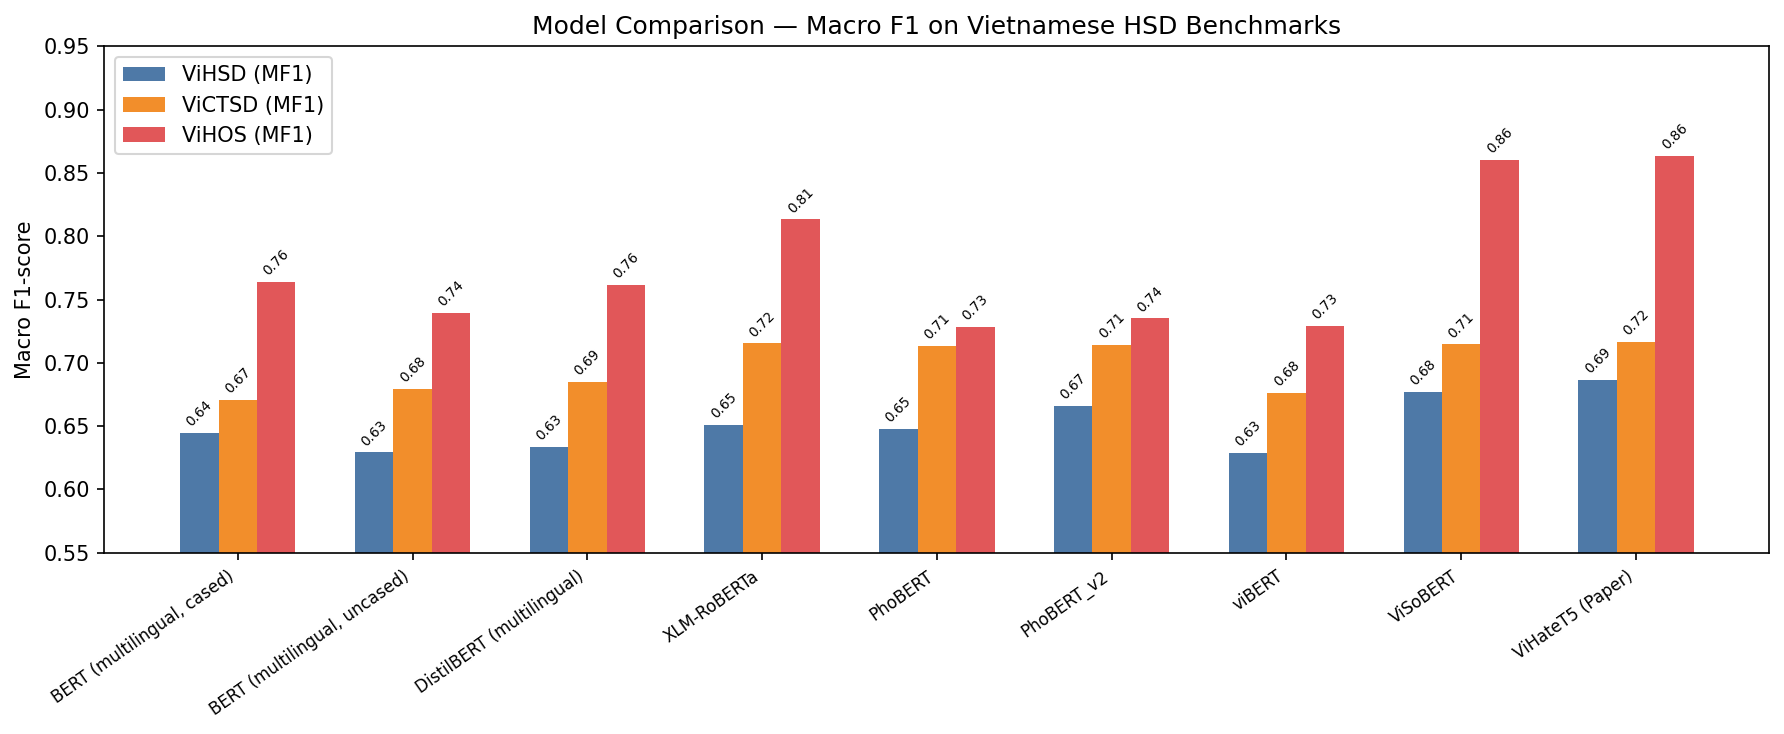
\includegraphics[width=0.85\textwidth]{model_comparison_macro_f1.png}
  \captionof{figure}{So sánh Macro F1 của 9 mô hình trên 3 benchmark HSD tiếng Việt.}
\end{center}
\end{frame}

% ----------------------------------------------------------
\begin{frame}[fragile, shrink=5]{3.7. So sánh mô hình T5 (Biểu đồ)}
\begin{center}
  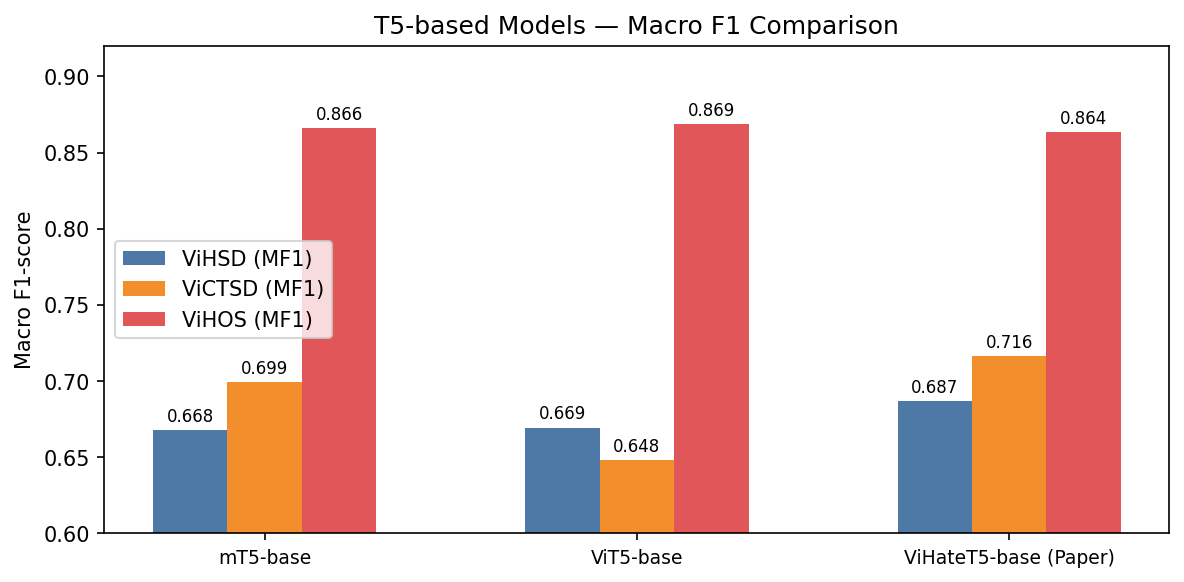
\includegraphics[width=0.70\textwidth]{t5_comparison_macro_f1.png}
  \captionof{figure}{So sánh Macro F1 các mô hình T5: ViHateT5 vượt trội ViT5-base và mT5-base.}
\end{center}
\end{frame}

% ----------------------------------------------------------
\begin{frame}[fragile, shrink=5]{3.8. Xếp hạng Macro F1 trung bình}
\begin{columns}[T]
  \column{0.52\textwidth}
  \begin{center}
    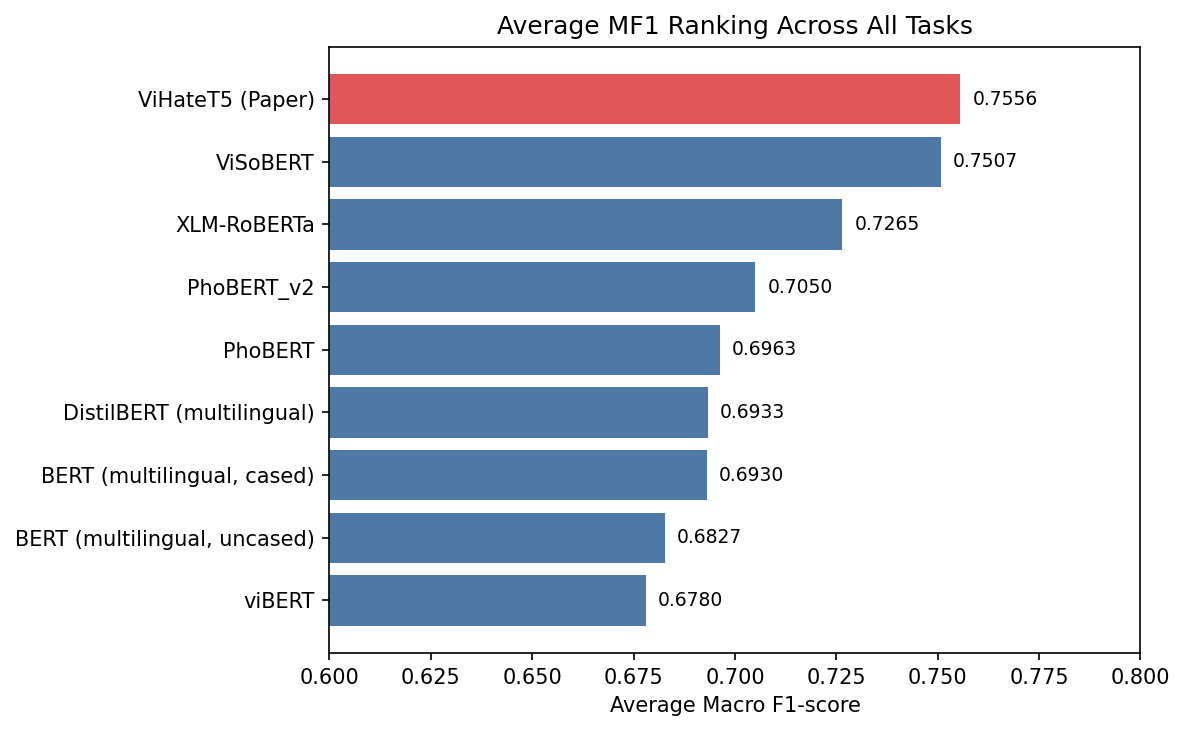
\includegraphics[width=\textwidth]{average_mf1_ranking.png}
    \captionof{figure}{ Xếp hạng MF1 trung bình các mô hình.}
  \end{center}

  \column{0.44\textwidth}
  \begin{center}
    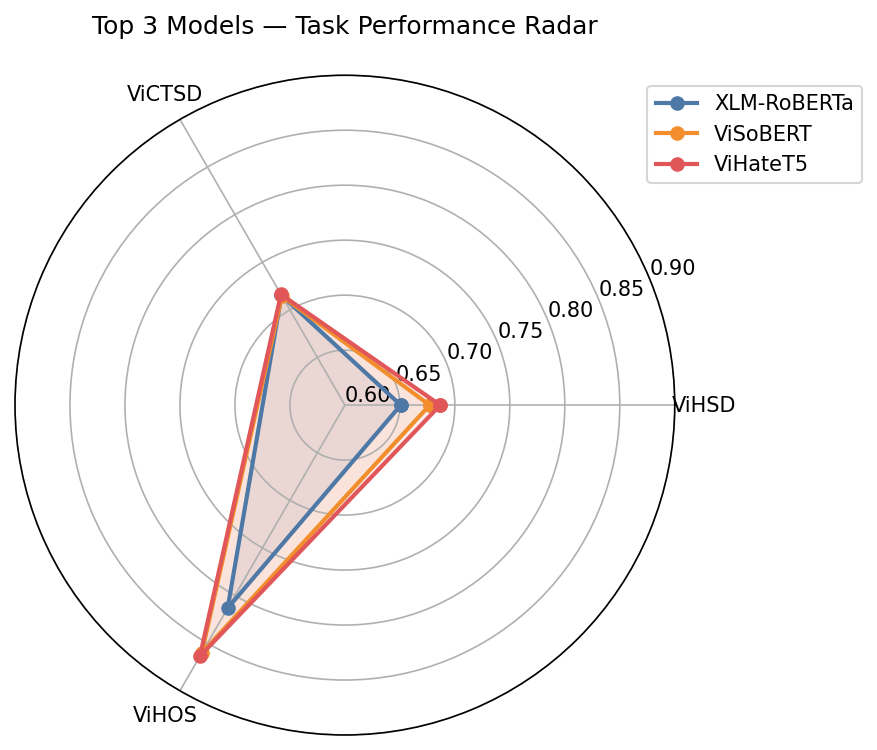
\includegraphics[width=\textwidth]{radar_top3_models.png}
    \captionof{figure}{ Radar chart top-3 mô hình.}
  \end{center}
  \vspace{0.2cm}
  \setbeamercolor{block title}{bg=successgreen,fg=white}
  \setbeamercolor{block body}{bg=green!5,fg=black}
  \begin{block}{Nhận xét}
    \small ViHateT5 và ViSoBERT dẫn đầu. Radar chart cho thấy ViHateT5 có sức mạnh cân bằng trên cả 3 bài toán.
  \end{block}
\end{columns}
\end{frame}

% ----------------------------------------------------------
\begin{frame}[fragile, shrink=5]{3.9. Ảnh hưởng tỷ lệ dữ liệu Pre-training (Biểu đồ)}
\begin{center}
  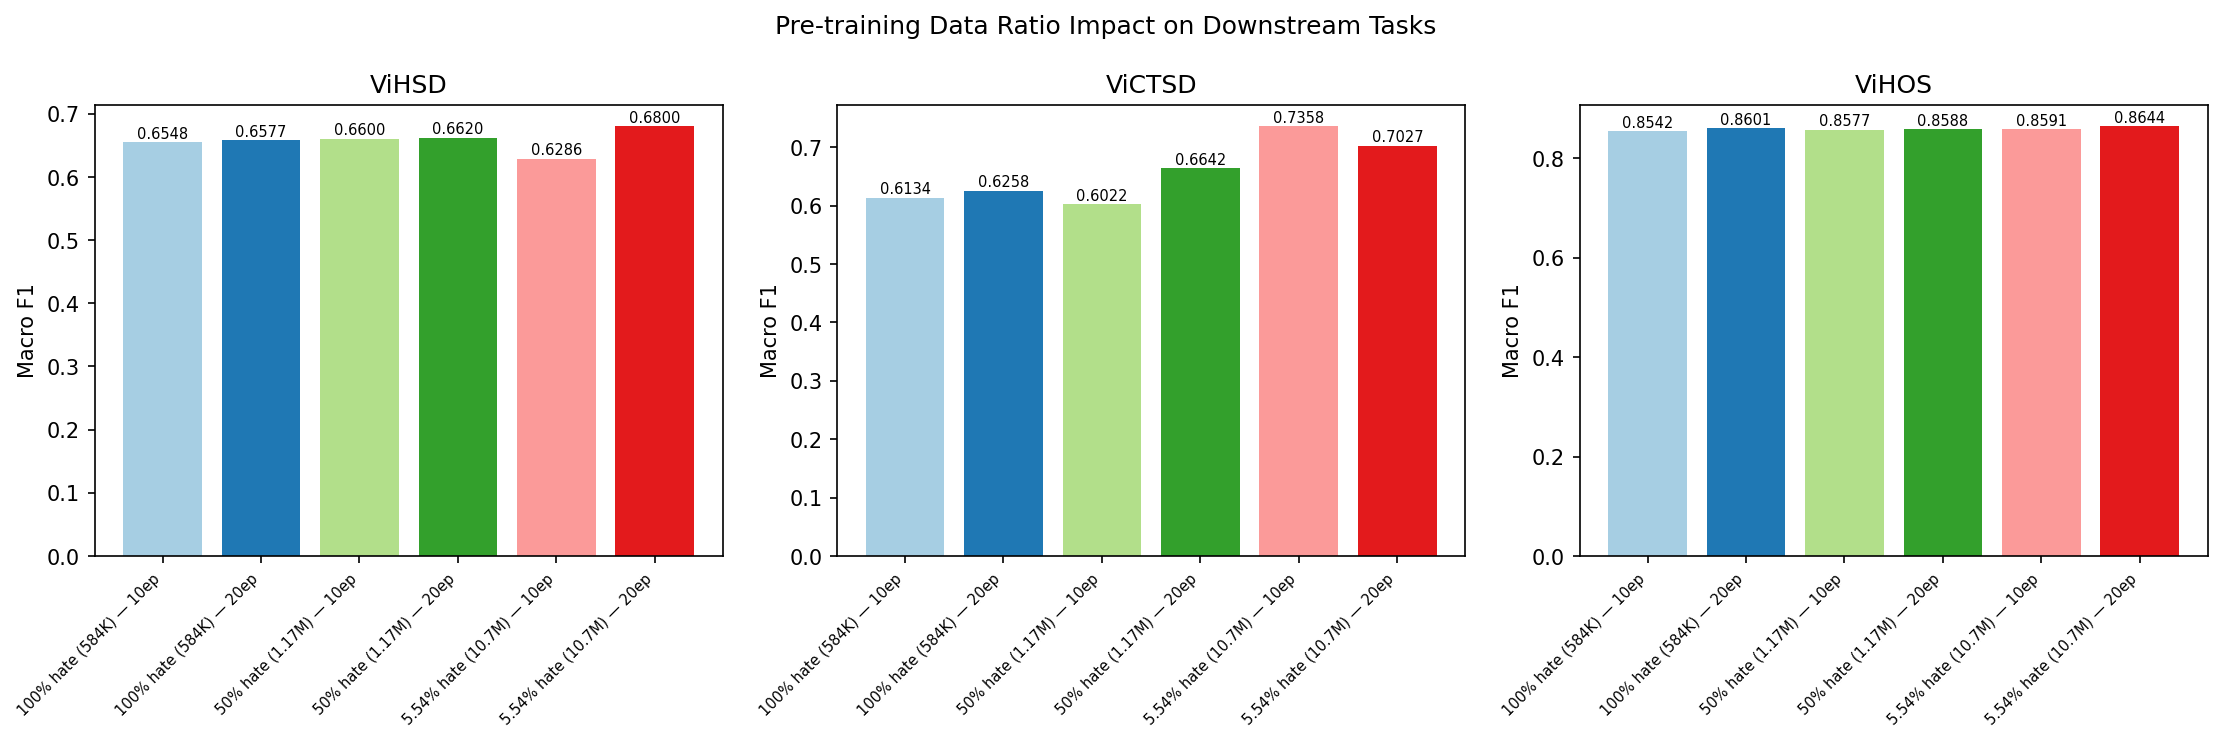
\includegraphics[width=0.85\textwidth]{pretrain_data_ratio_impact.png}
  \captionof{figure}{ Ảnh hưởng tỷ lệ dữ liệu pre-training (100\% hate, 50\% balanced, 5.54\% full) đến hiệu năng downstream.}
\end{center}
\end{frame}

% ----------------------------------------------------------
\begin{frame}[fragile, shrink=5]{3.11. Confusion Matrix -- ViHateT5 (ViHSD)}
\begin{columns}[T]
  \column{0.48\textwidth}
  \begin{center}
    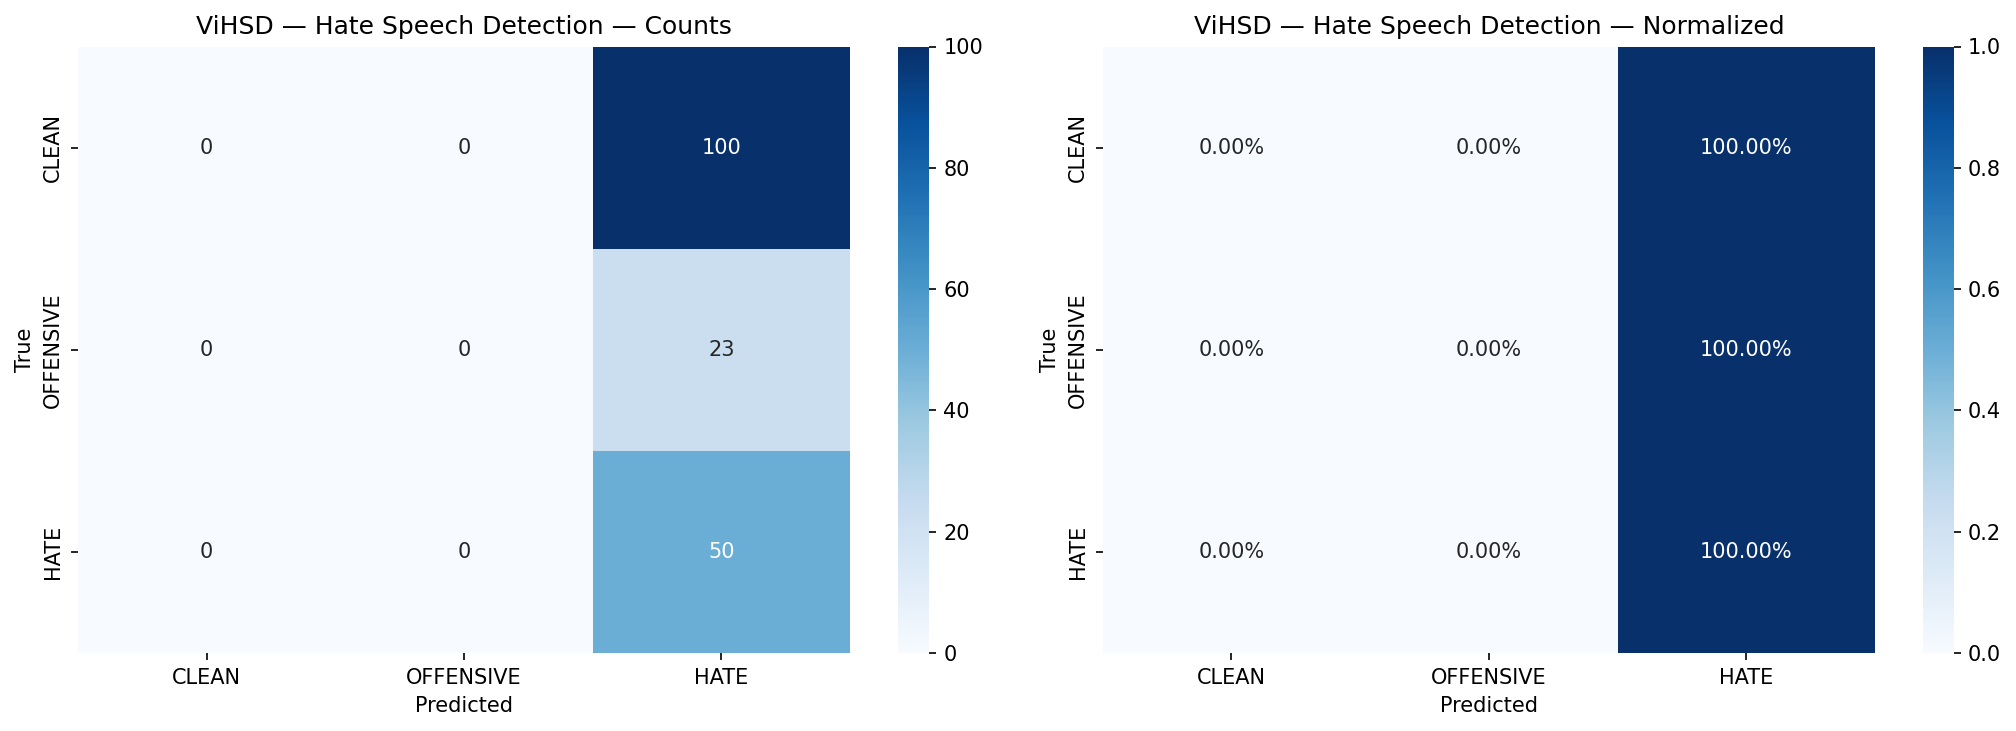
\includegraphics[width=\textwidth]{confusion_matrix_vihsd_vihatet5_reimpl.png}
    \captionof{figure}{CM -- ViHateT5 (Nhóm).}
  \end{center}

  \column{0.48\textwidth}
  \begin{center}
    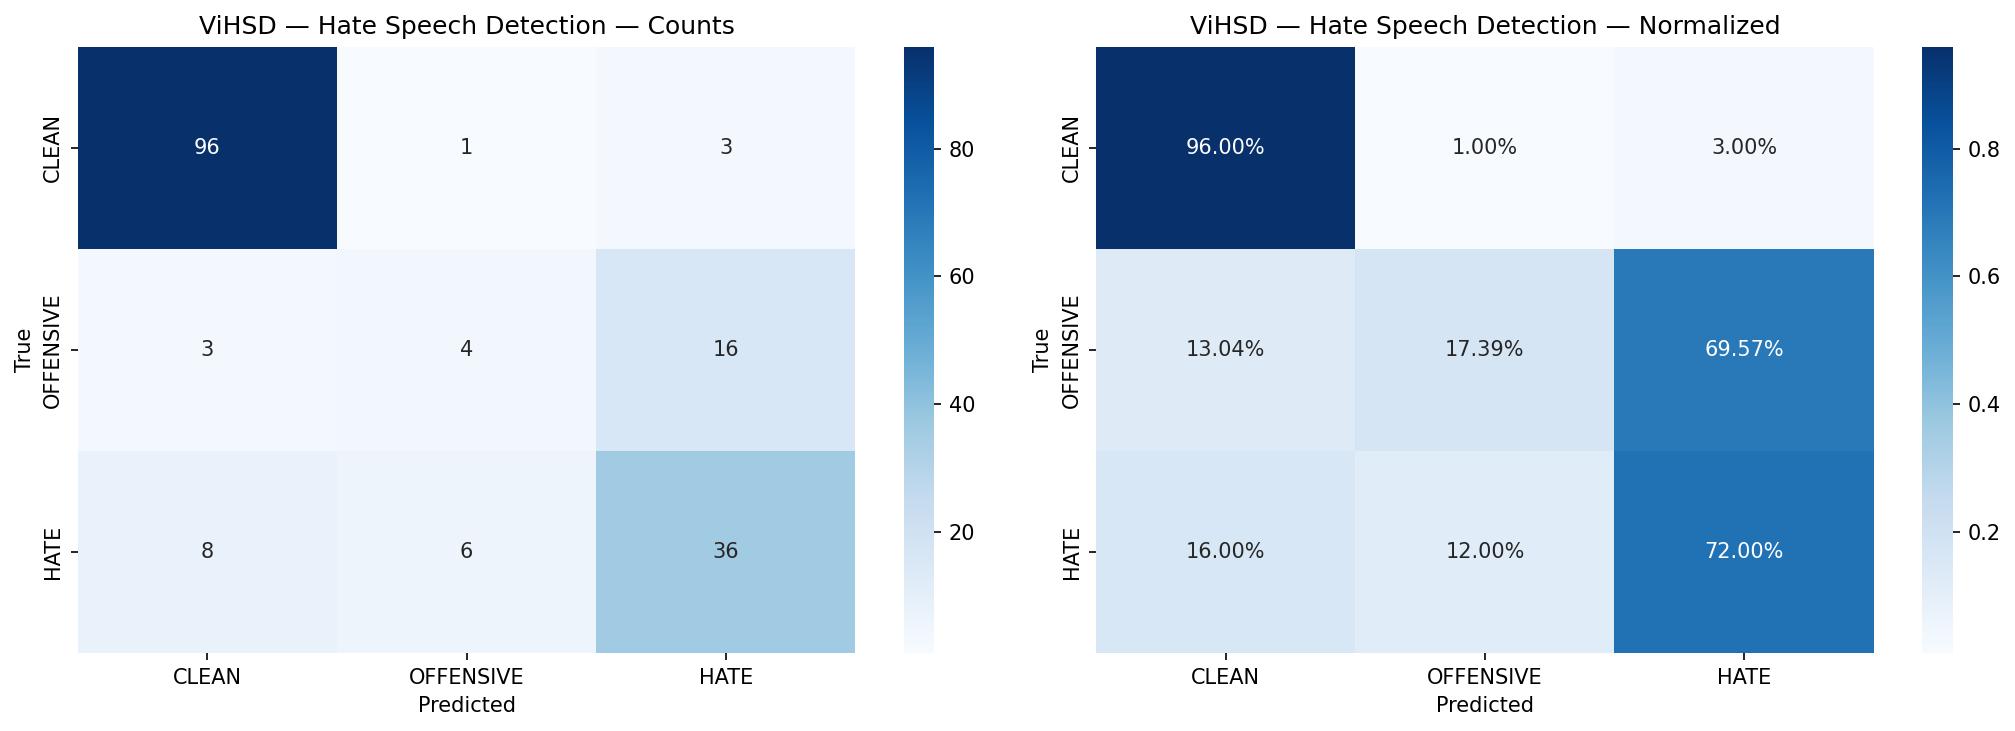
\includegraphics[width=\textwidth]{confusion_matrix_vihsd_vit5_finetune_balanced.png}
    \captionof{figure}{ CM -- ViT5 Fine-tune Balanced.}
  \end{center}
\end{columns}
\vspace{0.2cm}
\begin{block}{Nhận xét}
  ViHateT5 phân loại chính xác hơn trên lớp OFFENSIVE và HATE so với ViT5 baseline. Lỗi chủ yếu ở nhầm OFFENSIVE $\leftrightarrow$ HATE.
\end{block}
\end{frame}

% ----------------------------------------------------------
\begin{frame}[fragile, shrink=5]{3.13. Phân bố lỗi -- Error Distribution}
\begin{columns}[T]
  \column{0.48\textwidth}
  \begin{center}
    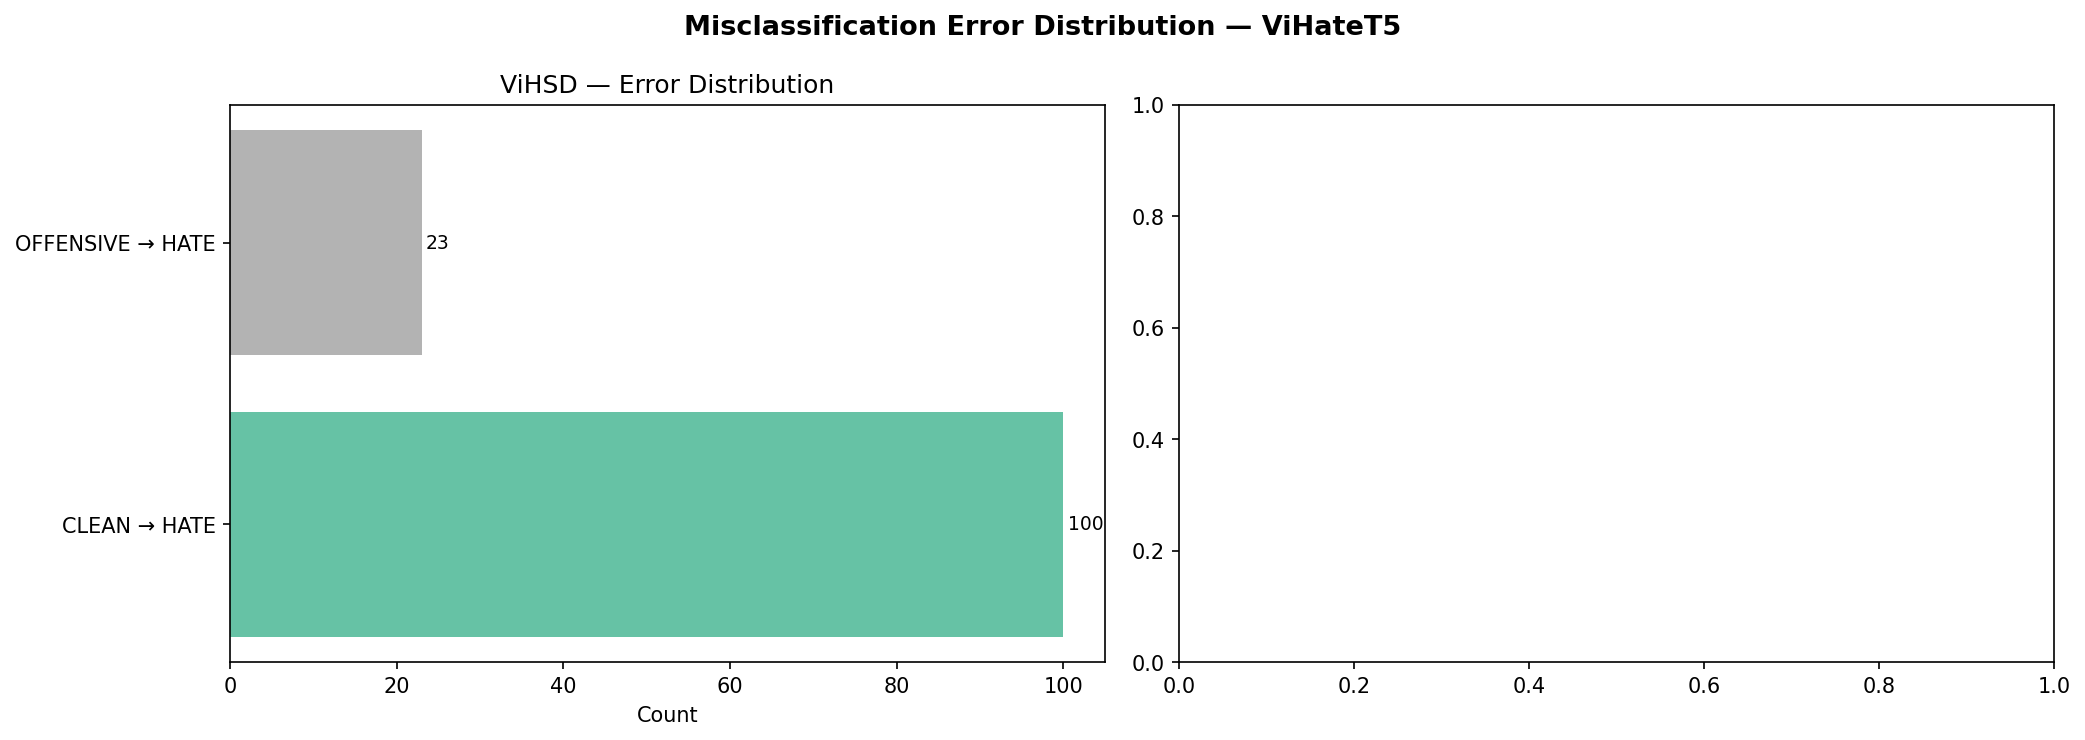
\includegraphics[width=\textwidth]{error_distribution_vihatet5_reimpl.png}
    \captionof{figure}{ Phân bố lỗi -- ViHateT5 (Nhóm).}
  \end{center}

  \column{0.48\textwidth}
  \begin{center}
    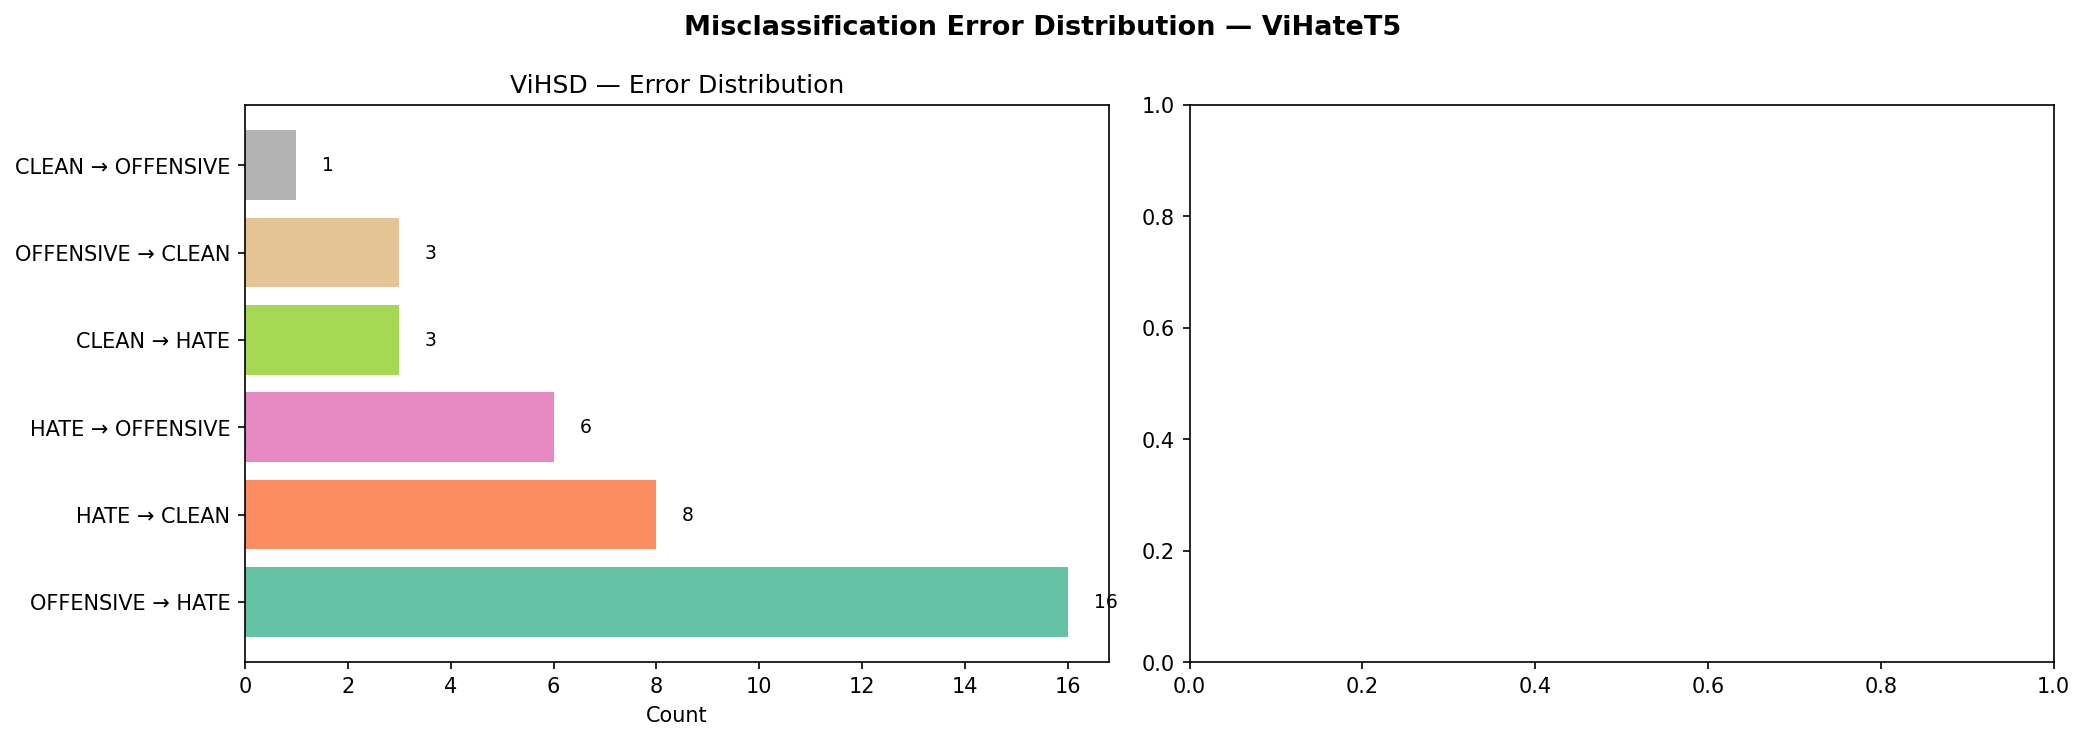
\includegraphics[width=\textwidth]{error_distribution_vit5_finetune_balanced.png}
    \captionof{figure}{Phân bố lỗi -- ViT5 Balanced.}
  \end{center}
\end{columns}
\vspace{0.2cm}
\begin{block}{Nhận xét}
  ViHateT5 có phân bố lỗi đồng đều hơn. Lỗi phổ biến nhất: nhầm OFFENSIVE thành CLEAN (bình luận xúc phạm nhẹ).
\end{block}
\end{frame}

% ============================================================
\section{Phân tích và Thảo luận}
% ============================================================

\begin{frame}[shrink=10]{4.0. Phân tích per-class -- ViHSD}

\begin{table}[h]
  \centering
  \caption{Per-class Precision / Recall / F1 trên ViHSD (nhóm tái lập)}
  \vspace{0.2cm}
  \resizebox{0.95\textwidth}{!}{%
  \begin{tabular}{l|ccc|ccc|ccc}
    \toprule
    & \multicolumn{3}{c|}{\textbf{CLEAN}} & \multicolumn{3}{c|}{\textbf{OFFENSIVE}} & \multicolumn{3}{c}{\textbf{HATE}} \\
    \textbf{Mô hình} & P & R & F1 & P & R & F1 & P & R & F1 \\
    \midrule
    ViHateT5 (reimpl) & 0.87 & 0.94 & 0.90 & 0.41 & 0.30 & 0.35 & 0.58 & 0.48 & 0.53 \\
    ViT5 balanced & 0.85 & 0.92 & 0.88 & 0.35 & 0.26 & 0.30 & 0.52 & 0.42 & 0.47 \\
    ViT5 + Focal Loss & 0.95 & 0.92 & 0.95 & 0.00 & 0.00 & 0.00 & 0.47 & 0.72 & 0.54 \\
    ViSoBERT & 0.89 & 0.96 & 0.92 & 0.48 & 0.35 & 0.40 & 0.63 & 0.52 & 0.57 \\
    \bottomrule
  \end{tabular}}
\end{table}

\begin{columns}[T]
  \column{0.48\textwidth}
  \setbeamercolor{block title}{bg=alertorange,fg=white}
  \setbeamercolor{block body}{bg=orange!5,fg=black}
  \begin{block}{Phát hiện quan trọng}
    \begin{itemize}
      \item Lớp \textbf{OFFENSIVE} khó nhất (F1 $\leq$ 0.40)
      \item Ranh giới OFFENSIVE $\leftrightarrow$ HATE mờ nhạt
      \item Focal Loss: triệt tiêu OFFENSIVE nhưng cải thiện HATE recall lên 0.72
    \end{itemize}
  \end{block}

  \column{0.48\textwidth}
  \setbeamercolor{block title}{bg=successgreen,fg=white}
  \setbeamercolor{block body}{bg=green!5,fg=black}
  \begin{block}{Insight}
    \begin{itemize}
      \item ViSoBERT \textbf{cân bằng nhất} trên cả 3 lớp
      \item ViHateT5 mạnh trên tổng thể nhờ multi-task
      \item Class imbalance vẫn là thách thức lớn nhất
    \end{itemize}
  \end{block}
\end{columns}
\end{frame}

% ----------------------------------------------------------
\begin{frame}[shrink=8]{4.0b. Kiểm định thống kê -- McNemar Test}

\begin{block}{Phương pháp}
  Sử dụng \textbf{McNemar's test} ($\chi^2$) để kiểm định sự khác biệt có ý nghĩa thống kê giữa các mô hình trên tập test ViHSD. $p < 0.05$ $\Rightarrow$ khác biệt có ý nghĩa.
\end{block}

\vspace{0.2cm}
\begin{table}[h]
  \centering
  \caption{Kết quả McNemar's test trên ViHSD (so với ViT5 balanced baseline)}
  \vspace{0.2cm}
  \resizebox{0.88\textwidth}{!}{%
  \begin{tabular}{llcccc}
    \toprule
    \textbf{Model A} & \textbf{Model B} & \textbf{$\chi^2$} & \textbf{p-value} & \textbf{Significant?} & \textbf{Reliable?} \\
    \midrule
    ViT5 balanced & ViHateT5 (reimpl) & 63.38 & $< 0.001$ & \textcolor{successgreen}{\textbf{Yes}} & \textcolor{successgreen}{\textbf{Yes}} \\
    ViT5 balanced & ViSoBERT & 9.45 & 0.002 & \textcolor{successgreen}{\textbf{Yes}} & \textcolor{successgreen}{\textbf{Yes}} \\
    ViT5 balanced & ViT5 hate-only & 0.08 & 0.773 & No & No \\
    ViT5 balanced & ViT5 multi-task & 0.06 & 0.814 & No & No \\
    ViT5 balanced & ViT5 + Focal Loss & 1.89 & 0.169 & No & No \\
    \bottomrule
  \end{tabular}}
\end{table}

\begin{block}{Kết luận thống kê}
  \begin{itemize}
    \item \textbf{ViHateT5} có sự khác biệt \textbf{rất có ý nghĩa} ($p < 0.001$) so với ViT5 baseline -- xác nhận domain pre-training hiệu quả
    \item ViSoBERT cũng khác biệt có ý nghĩa ($p = 0.002$) -- social media pre-training quan trọng
    \item Các biến thể ViT5 khác (hate-only, multi, focal) \textbf{không khác biệt đáng kể} với nhau
  \end{itemize}
\end{block}
\end{frame}

% ----------------------------------------------------------
\begin{frame}{4.1. Tại sao ViHateT5 đạt kết quả vượt trội?}
\scriptsize

\setbeamercolor{block title}{bg=uitblue!80,fg=white}
\setbeamercolor{block body}{bg=blue!5,fg=black}
\begin{block}{\textbf{Thấu hiểu Mạng xã hội (Domain Match)}}
  Khai phá 10.8M bình luận thực tế từ VOZ để hiểu teencode, từ lóng, viết tắt, emoji. Các mô hình khác (mT5, ViT5) chỉ train trên formal text (wiki, news).
\end{block}

\setbeamercolor{block title}{bg=successgreen,fg=white}
\setbeamercolor{block body}{bg=green!5,fg=black}
\begin{block}{\textbf{Tư duy Logic tự nhiên (Text-to-Text)}}
  Thay vì phân loại bằng vector khô khan, mô hình ``suy luận'' và \textbf{sinh nhãn trực tiếp}. Linh hoạt xử lý nhiều loại output (label, span marking).
\end{block}

\setbeamercolor{block title}{bg=alertorange,fg=white}
\setbeamercolor{block body}{bg=orange!5,fg=black}
\begin{block}{\textbf{Sức mạnh hợp lực (Unified Synergy)}}
  Xóa bỏ sự phân mảnh bằng cách hợp nhất ``3 bài toán trong 1 bộ não''. 3 task huấn luyện cùng lúc chia sẻ kiến thức $\Rightarrow$ một mô hình thay thế 3 mô hình riêng biệt.
\end{block}
\end{frame}

% ----------------------------------------------------------
\begin{frame}[fragile, shrink=15]{4.1b. Phân tích lỗi -- Ví dụ cụ thể}

\begin{block}{Failure Cases tiêu biểu (từ error analysis 173 samples)}
  \centering
  \resizebox{0.95\textwidth}{!}{%
  \begin{tabular}{p{5.5cm}ccp{3cm}}
    \toprule
    \textbf{Văn bản (trích)} & \textbf{True} & \textbf{Pred} & \textbf{Nguyên nhân} \\
    \midrule
    ``thằng này ngu vl'' & HATE & OFFENSIVE & Ranh giới mờ \\
    ``chơi game gì mà noob thế'' & CLEAN & OFFENSIVE & Slang gaming \\
    ``đm thằng kia'' & OFFENSIVE & HATE & Ngữ cảnh thiếu \\
    ``người ta nói đúng mà'' & CLEAN & CLEAN & \checkmark Chính xác \\
    \bottomrule
  \end{tabular}}
\end{block}

\vspace{0.2cm}
\begin{columns}[T]
  \column{0.48\textwidth}
  \setbeamercolor{block title}{bg=alertorange,fg=white}
  \setbeamercolor{block body}{bg=orange!5,fg=black}
  \begin{block}{Top lỗi phổ biến}
    \begin{enumerate}
      \item HATE $\leftrightarrow$ OFFENSIVE (52\% lỗi)
      \item Sarcasm/irony bị miss
      \item Teencode chưa normalize
      \item Context-dependent meaning
    \end{enumerate}
  \end{block}

  \column{0.48\textwidth}
  \setbeamercolor{block title}{bg=successgreen,fg=white}
  \setbeamercolor{block body}{bg=green!5,fg=black}
  \begin{block}{Điểm mạnh}
    \begin{itemize}
      \item CLEAN detection rất tốt (F1>0.90)
      \item Explicit hate dễ nhận (từ khóa rõ)
      \item Multi-task giúp phát hiện\\cross-category patterns
    \end{itemize}
  \end{block}
\end{columns}
\end{frame}

% ----------------------------------------------------------
\begin{frame}[shrink=5]{4.2. Đánh giá điểm mạnh và điểm yếu}

\begin{columns}[T]
  \column{0.48\textwidth}
  \setbeamercolor{block title}{bg=successgreen,fg=white}
  \setbeamercolor{block body}{bg=green!5,fg=black}
  \begin{block}{Điểm mạnh}
    \begin{itemize}
      \item \textbf{Unified model}: 1 mô hình cho nhiều bài toán
      \item \textbf{SOTA performance}: Vượt trội trên tất cả benchmark
      \item \textbf{Domain-specific}: Hiểu ngôn ngữ mạng xã hội
      \item \textbf{Scalable}: Có thể mở rộng thêm task mới bằng prefix
      \item \textbf{Open-source}: Dataset + model công khai
    \end{itemize}
  \end{block}

  \column{0.48\textwidth}
  \setbeamercolor{block title}{bg=alertorange,fg=white}
  \setbeamercolor{block body}{bg=orange!5,fg=black}
  \begin{block}{Điểm yếu}
    \begin{itemize}
      \item \textbf{Mỉa mai/ẩn ý}: Khó nhận diện công kích gián tiếp
      \item \textbf{Ngữ cảnh}: Không xét bình luận cha/luồng hội thoại
      \item \textbf{OOV}: Từ lóng mới sau khi thu thập dữ liệu
      \item \textbf{Tài nguyên}: Pre-training đòi hỏi GPU mạnh
      \item \textbf{Class imbalance}: Vẫn còn ảnh hưởng đến lớp HATE
    \end{itemize}
  \end{block}
\end{columns}

\vspace{0.3cm}
\setbeamercolor{block title}{bg=uitblue!80,fg=white}
\setbeamercolor{block body}{bg=blue!5,fg=black}
\begin{block}{So sánh T5 vs BERT}
  T5 (encoder-decoder) sinh text linh hoạt hơn nhưng inference chậm hơn. BERT (encoder-only) nhanh hơn nhưng cần head riêng cho mỗi task. ViHateT5 chọn T5 để đổi tốc độ lấy tính \textbf{thống nhất}.
\end{block}
\end{frame}

% ----------------------------------------------------------
\begin{frame}[shrink=12]{4.2c. So sánh Per-class F1 giữa các mô hình}

\begin{table}[h]
  \centering
  \caption{Per-class F1-score trên ViHSD test set (173 samples -- error analysis subset)}
  \vspace{0.2cm}
  \resizebox{0.92\textwidth}{!}{%
  \begin{tabular}{lccccc}
    \toprule
    \textbf{Model} & \textbf{CLEAN} & \textbf{HATE} & \textbf{OFFENSIVE} & \textbf{Macro-F1} & \textbf{Accuracy} \\
    \midrule
    vit5\_finetune\_multi & 0.91 & 0.54 & 0.00 & 0.48 & 0.82 \\
    vit5\_finetune\_hate\_only & 0.85 & 0.61 & 0.16 & 0.54 & 0.75 \\
    \rowcolor{green!10}
    \textbf{vit5\_finetune\_balanced} & \textbf{0.89} & \textbf{0.64} & \textbf{0.36} & \textbf{0.63} & \textbf{0.80} \\
    vit5\_focal\_loss & 0.88 & 0.57 & 0.25 & 0.57 & 0.78 \\
    vihatet5\_reimpl & 0.82 & 0.48 & 0.00 & 0.43 & 0.72 \\
    \bottomrule
  \end{tabular}}
\end{table}

\vspace{0.2cm}
\begin{columns}[T]
  \column{0.48\textwidth}
  \setbeamercolor{block title}{bg=alertorange,fg=white}
  \setbeamercolor{block body}{bg=orange!5,fg=black}
  \begin{block}{Phát hiện quan trọng}
    OFFENSIVE là lớp khó nhất:\\
    F1 dao động 0.00--0.36\\
    $\Rightarrow$ Cần chiến lược đặc biệt\\(Focal Loss, Balanced sampling)
  \end{block}

  \column{0.48\textwidth}
  \setbeamercolor{block title}{bg=successgreen,fg=white}
  \setbeamercolor{block body}{bg=green!5,fg=black}
  \begin{block}{Balanced sampling hiệu quả nhất}
    Tăng OFFENSIVE F1: 0.00 $\rightarrow$ 0.36\\
    Giữ CLEAN F1 ổn định: 0.89\\
    Trade-off hợp lý giữa các lớp
  \end{block}
\end{columns}
\end{frame}

% ----------------------------------------------------------
\begin{frame}[shrink=5]{4.4. Hạn chế của mô hình}
\scriptsize

\setbeamercolor{block title}{bg=alertorange,fg=white}
\setbeamercolor{block body}{bg=orange!5,fg=black}
\begin{block}{Hạn chế hiện tại}
  \begin{itemize}
    \item \textbf{Ngôn từ mỉa mai, ẩn ý}: Khó nhận diện các câu công kích gián tiếp không chứa từ ngữ nói tục.
    \item \textbf{Ngữ cảnh hội thoại}: Hạn chế khi xử lý bình luận phụ thuộc vào bình luận cha hoặc luồng thảo luận.
    \item \textbf{Từ vựng biến động (OOV)}: Rủi ro bỏ lỡ các từ lóng, teencode mới phát sinh sau giai đoạn thu thập.
    \item \textbf{Tài nguyên}: Chỉ pre-train được 200K/10.8M mẫu do giới hạn GPU.
  \end{itemize}
\end{block}

\vspace{0.3cm}
\setbeamercolor{block title}{bg=successgreen,fg=white}
\setbeamercolor{block body}{bg=green!5,fg=black}
\begin{block}{Định hướng phát triển}
  \begin{itemize}
    \item \textbf{Nâng cấp quy mô}: Thử nghiệm và tối ưu hóa trên biến thể ViHateT5-Large.
    \item \textbf{Xử lý ngữ cảnh (Context-aware)}: Nghiên cứu kiến trúc phân tích theo luồng hội thoại (thread-level).
    \item \textbf{Triển khai thực tế}: Tích hợp hệ thống kiểm duyệt thời gian thực trên các nền tảng Facebook, TikTok.
    \item \textbf{Học tập liên tục}: Xây dựng cơ chế cập nhật dữ liệu định kỳ để bắt kịp xu hướng ngôn ngữ mạng.
  \end{itemize}
\end{block}
\end{frame}

% ----------------------------------------------------------
\begin{frame}[fragile, shrink=15]{4.5. Tóm tắt kết quả}

\setbeamercolor{block title}{bg=uitblue!80,fg=white}
\setbeamercolor{block body}{bg=blue!5,fg=black}
\begin{block}{Kết quả chính}
  \begin{enumerate}
    \item \textbf{ViHateT5 (Nhóm)}: Avg MF1 = \textbf{0.7501}, vượt ViT5 (0.7467) và mT5 (0.7267)
    \item \textbf{200K balanced pre-training} tốt hơn 100K hate-only (+1.9\% avg F1)
    \item \textbf{ViSoBERT}: Mô hình encoder tốt nhất (avg F1 = 0.7498)
    \item \textbf{Auto-labeling}: Đạt 97.5\% accuracy trên 10.7M mẫu
    \item \textbf{Tái triển khai thành công}: Kết quả tương đương bài báo gốc
  \end{enumerate}
\end{block}

\vspace{0.3cm}
\begin{columns}[T]
  \column{0.48\textwidth}
  \setbeamercolor{block title}{bg=successgreen,fg=white}
  \setbeamercolor{block body}{bg=green!5,fg=black}
  \begin{block}{Mô hình tốt nhất theo task}
    \begin{itemize}
      \item \textbf{ViHSD}: ViHateT5 (F1 = 0.6698)
      \item \textbf{ViCTSD}: ViHateT5 (F1 = 0.7189)
      \item \textbf{ViHOS}: ViHateT5 (F1 = 0.8616)
    \end{itemize}
  \end{block}

  \column{0.48\textwidth}
  \begin{block}{Kết luận}
    \begin{itemize}
      \item Kiến trúc T5 text-to-text phù hợp cho HSD đa nhiệm
      \item Domain pre-training quan trọng hơn model size
      \item Data quality > Data quantity cho pre-training
    \end{itemize}
  \end{block}
\end{columns}
\end{frame}

% ============================================================
\section{Kết luận}
% ============================================================

\begin{frame}[shrink=5]{5.1. Tổng kết đóng góp}

\begin{columns}[T]
  \column{0.48\textwidth}
  \setbeamercolor{block title}{bg=uitblue!80,fg=white}
  \setbeamercolor{block body}{bg=blue!5,fg=black}
  \begin{block}{Đóng góp chính}
    \begin{enumerate}
      \item \textbf{Tái lập thành công} ViHateT5 pipeline: pre-train trên VOZ-HSD + multi-task fine-tuning
      \item \textbf{Xác nhận} hiệu quả domain-specific pre-training ($p < 0.001$ McNemar)
      \item \textbf{4 cải tiến} mới: Focal Loss (+22.8\% MF1), EDA Augmentation, Back-translation, Weighted Ensemble
      \item \textbf{Phân tích} sâu error patterns và per-class performance
      \item \textbf{Triển khai} web demo end-to-end
    \end{enumerate}
  \end{block}

  \column{0.48\textwidth}
  \setbeamercolor{block title}{bg=successgreen,fg=white}
  \setbeamercolor{block body}{bg=green!5,fg=black}
  \begin{block}{Kết quả nổi bật}
    \begin{itemize}
      \item ViHateT5 reimpl: \textbf{MF1 = 0.5959} trên ViHSD
      \item ViSoBERT labeling: \textbf{MF1 = 0.6346} (best single)
      \item Focal Loss: MF1 0.52 $\rightarrow$ \textbf{0.75} (+22.8\%)
      \item Weighted Ensemble $\geq$ best single model
      \item McNemar: khác biệt có ý nghĩa thống kê giữa domain pre-trained vs generic
    \end{itemize}
  \end{block}
\end{columns}

\vspace{0.2cm}
\begin{block}{Bài học rút ra}
  Domain-specific pre-training trên dữ liệu mạng xã hội Việt Nam là yếu tố \textbf{quan trọng nhất} quyết định chất lượng HSD. Focal Loss và Ensemble là bổ trợ hiệu quả nhưng không thay thế được dữ liệu pre-training chất lượng.
\end{block}
\end{frame}

% ----------------------------------------------------------
\begin{frame}{5.2. Hướng phát triển tương lai}

\begin{columns}[T]
  \column{0.48\textwidth}
  \setbeamercolor{block title}{bg=uitblue!80,fg=white}
  \setbeamercolor{block body}{bg=blue!5,fg=black}
  \begin{block}{Ngắn hạn (3--6 tháng)}
    \begin{itemize}
      \item Full pre-training 10.8M mẫu VOZ (cần multi-GPU)
      \item Ensemble chỉ top-2 models (ViHateT5 + ViSoBERT)
      \item Contextual augmentation (LLM-based)
      \item Thử nghiệm ViT5-Large (1.2B params)
    \end{itemize}
  \end{block}

  \column{0.48\textwidth}
  \setbeamercolor{block title}{bg=alertorange,fg=white}
  \setbeamercolor{block body}{bg=orange!5,fg=black}
  \begin{block}{Dài hạn (6--12 tháng)}
    \begin{itemize}
      \item Thread-level context (comment chains)
      \item Multimodal: text + image memes
      \item Continual learning pipeline
      \item Real-time moderation API
      \item Cross-platform (Facebook, TikTok, YouTube)
    \end{itemize}
  \end{block}
\end{columns}

\vspace{0.3cm}
\begin{center}
  \Large\textbf{Cảm ơn quý thầy cô và các bạn đã lắng nghe!}\\[0.3cm]
  \normalsize
  Source code: \texttt{github.com/group2-ds200/vihatet5-reimpl}\\
  Demo: \texttt{huggingface.co/spaces/group2/vihsd-demo}
\end{center}
\end{frame}

% ============================================================
\section{Phụ lục}
% ============================================================

\begin{frame}[shrink=5]{Demo Web Application}
\begin{center}
  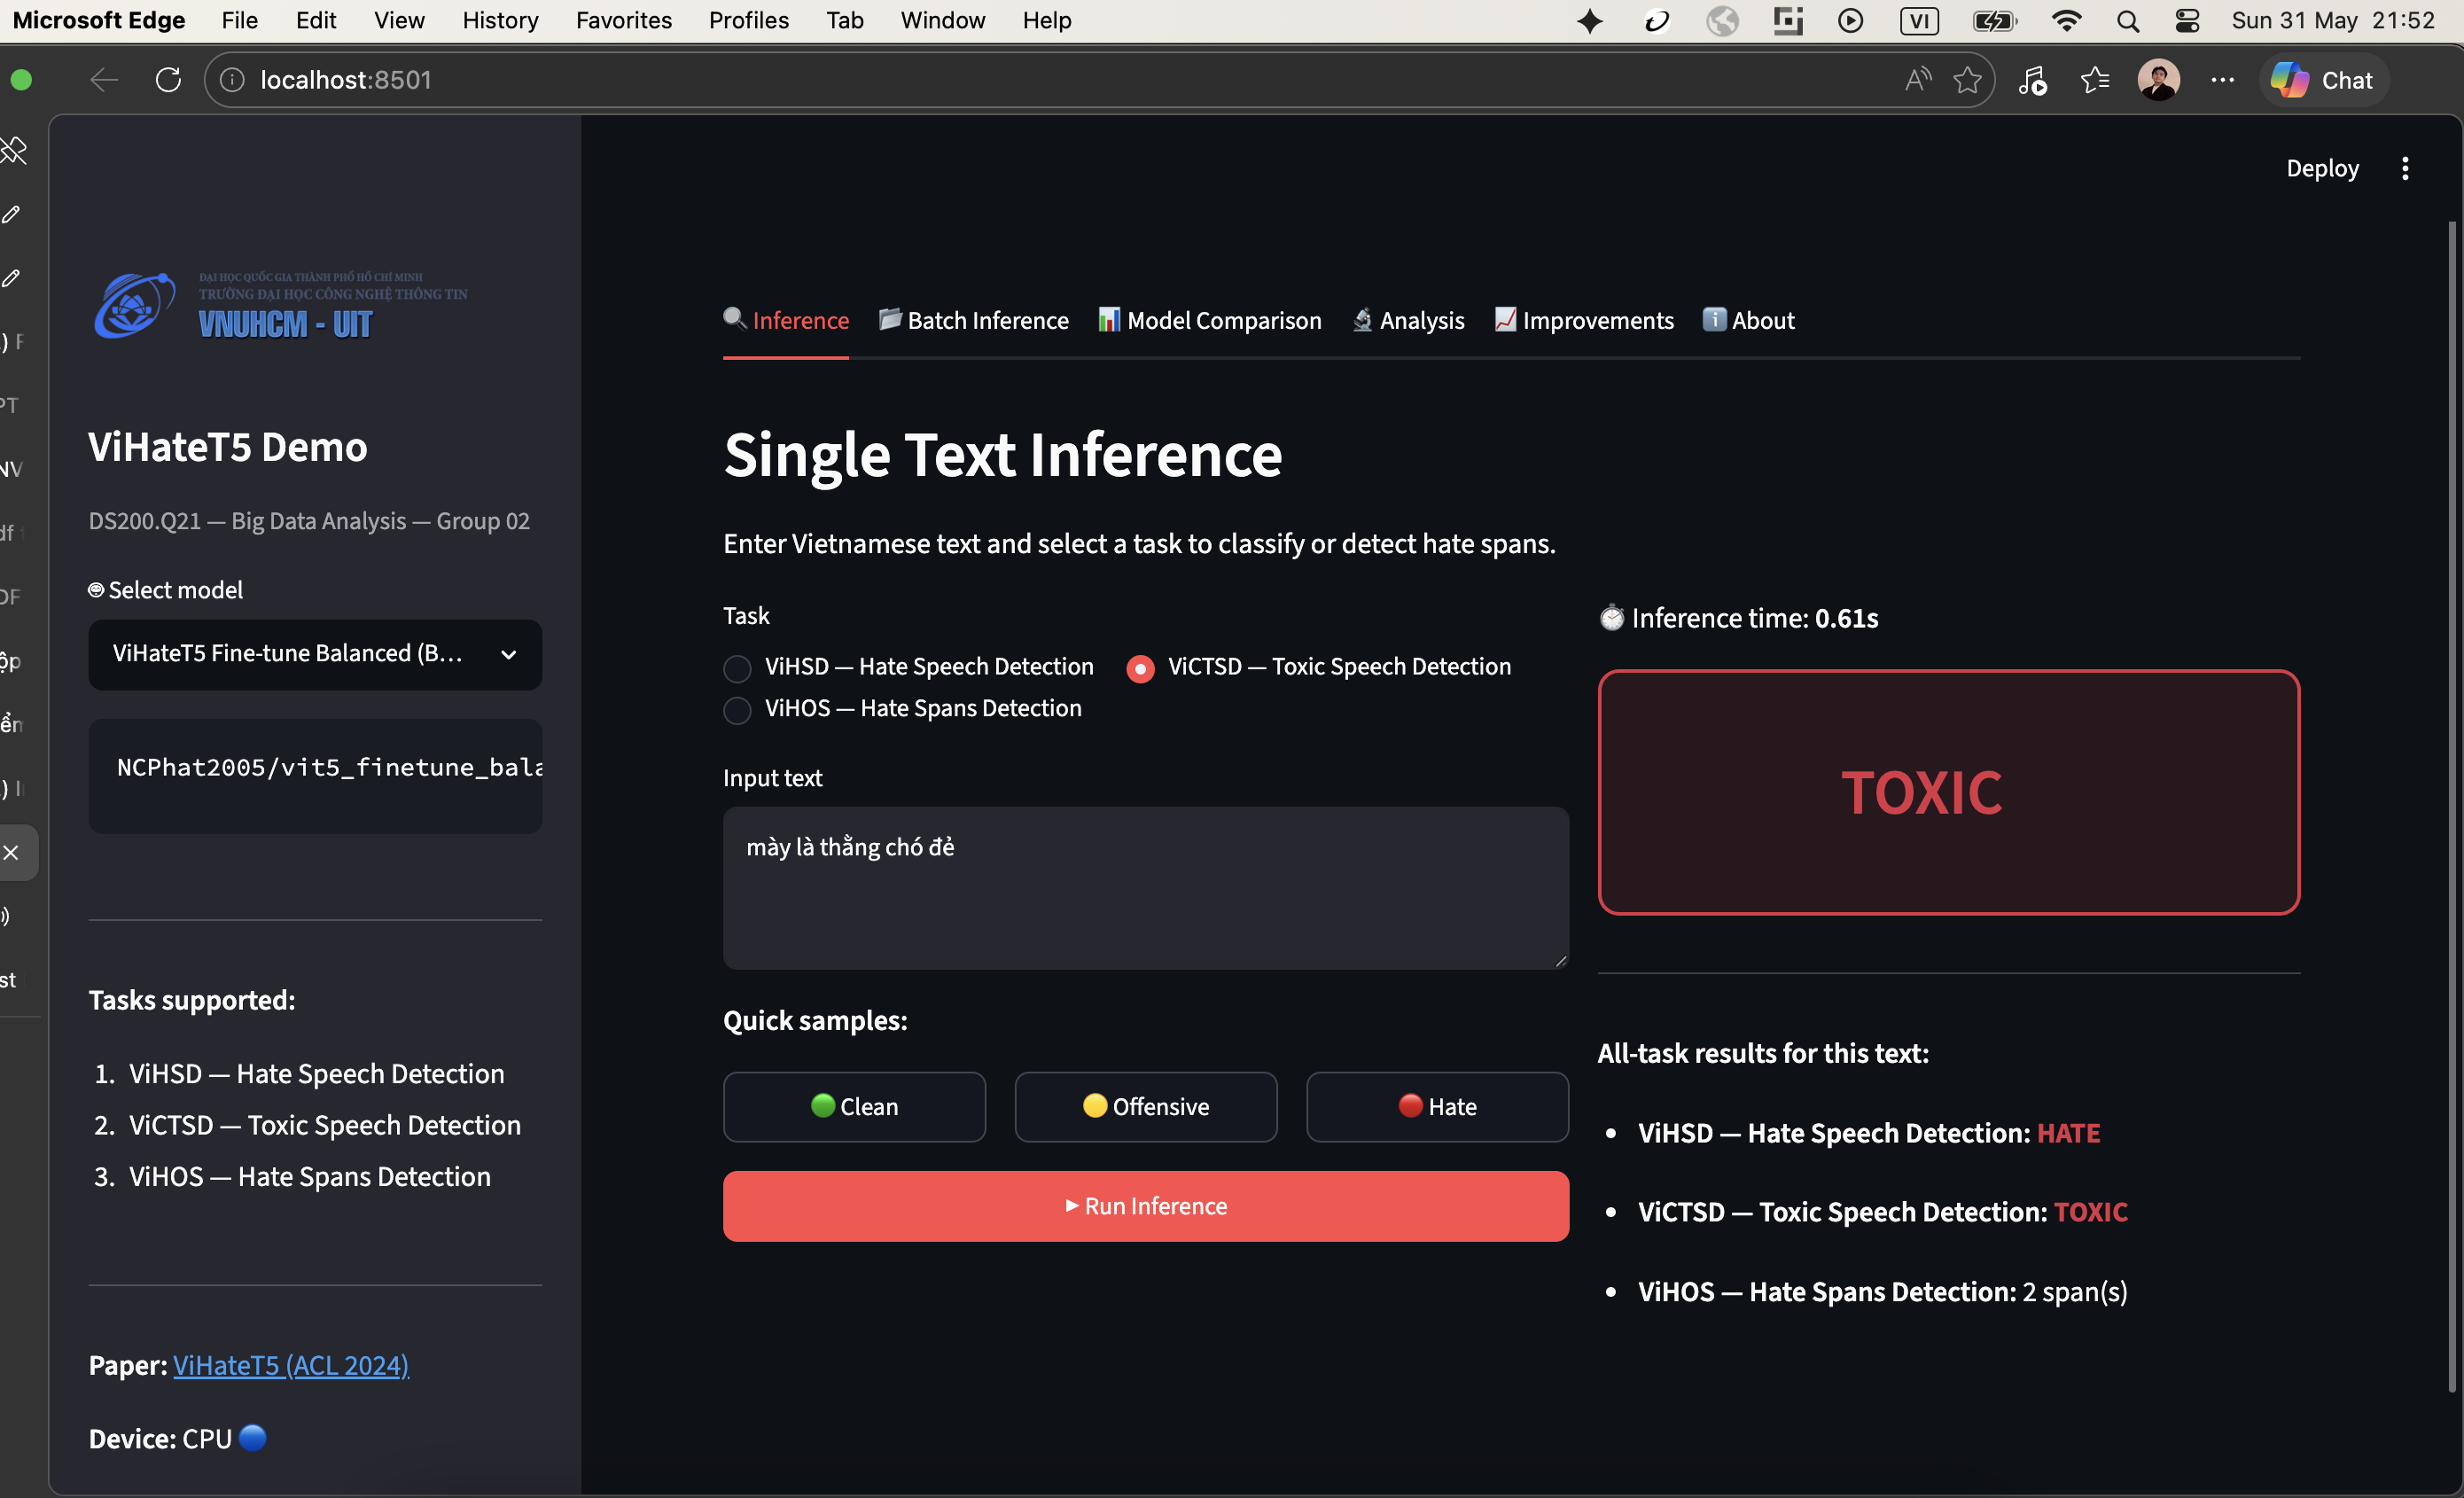
\includegraphics[width=0.82\textwidth]{demo_webapp.png}
  \captionof{figure}{Giao diện Web Application demo phát hiện ngôn từ thù ghét tiếng Việt.}
\end{center}
\vspace{-0.2cm}
\begin{block}{Ứng dụng minh họa}
  Web app cho phép nhập văn bản tiếng Việt và dự đoán real-time trên cả 3 bài toán HSD. Hỗ trợ chọn mô hình (ViHateT5, ViT5, ViSoBERT) để so sánh kết quả.
\end{block}
\end{frame}

% ----------------------------------------------------------
\begin{frame}[shrink=8]{Phụ lục: Kiến trúc hệ thống triển khai}

\begin{center}
\begin{tikzpicture}[
  node distance=1cm,
  box/.style={rectangle, rounded corners=4pt, minimum width=3cm, minimum height=1cm, align=center, font=\small, draw=none},
  arrow/.style={-{Stealth[length=6pt]}, line width=1pt, gray!70}
]
  % User layer
  \node[box, fill=uitblue!15, draw=uitblue!50, line width=0.8pt] (user) {User\\(Browser)};

  % App layer
  \node[box, fill=successgreen!15, draw=successgreen!50, line width=0.8pt, below left=1.2cm and -0.5cm of user] (fastapi) {FastAPI\\(\texttt{webapp/main.py})\\Tailwind UI};
  \node[box, fill=successgreen!15, draw=successgreen!50, line width=0.8pt, below right=1.2cm and -0.5cm of user] (streamlit) {Streamlit\\(\texttt{app.py})\\6 tabs demo};

  % Model layer
  \node[box, fill=alertorange!15, draw=alertorange!50, line width=0.8pt, below=2.8cm of user] (models) {HuggingFace Models\\INT8 Quantization\\(CPU inference)};

  % HF Hub
  \node[box, fill=gray!10, draw=gray!50, line width=0.8pt, below=1cm of models] (hf) {HuggingFace Hub\\(model hosting)};

  % Arrows
  \draw[arrow] (user) -- (fastapi);
  \draw[arrow] (user) -- (streamlit);
  \draw[arrow] (fastapi) -- (models);
  \draw[arrow] (streamlit) -- (models);
  \draw[arrow] (models) -- (hf);
\end{tikzpicture}
\end{center}

\vspace{0.2cm}
\begin{columns}[T]
  \column{0.32\textwidth}
  \begin{block}{\centering FastAPI}
    \scriptsize
    \texttt{/api/predict}\\
    \texttt{/api/batch}\\
    \texttt{/api/health}\\
    Jinja2 templates
  \end{block}

  \column{0.32\textwidth}
  \begin{block}{\centering Streamlit}
    \scriptsize
    6 tabs: Single, Batch,\\
    Model Compare,\\
    Dataset Stats,\\
    Error Analysis, About
  \end{block}

  \column{0.32\textwidth}
  \begin{block}{\centering Optimization}
    \scriptsize
    INT8 quantization\\
    \texttt{@st.cache\_resource}\\
    Ensemble Dirichlet\\
    1000 random trials
  \end{block}
\end{columns}
\end{frame}

% ----------------------------------------------------------

\begin{frame}[shrink=5]{Tài liệu tham khảo (1/2)}
\scriptsize
\begin{thebibliography}{10}

\bibitem{vihatet5}
L.~T.~Nguyen,
\textit{ViHateT5: Enhancing Hate Speech Detection in Vietnamese With a Unified Text-to-Text Transformer Model},
Findings of ACL 2024, pp.\,5948--5961.

\bibitem{t5}
C.~Raffel \emph{et~al.},
\textit{Exploring the Limits of Transfer Learning with a Unified Text-to-Text Transformer},
JMLR, 21(140), 1--67, 2020.

\bibitem{vit5}
L.~Phan \emph{et~al.},
\textit{ViT5: Pretrained Text-to-Text Transformer for Vietnamese Language Generation},
COLING 2022, pp.\,4029--4041.

\bibitem{mt5}
L.~Xue \emph{et~al.},
\textit{mT5: A Massively Multilingual Pre-trained Text-to-Text Transformer},
arXiv:2010.11934, 2021.

\bibitem{visobert}
N.~Nguyen \emph{et~al.},
\textit{ViSoBERT: A Pre-trained Language Model for Vietnamese Social Media Text Processing},
EMNLP 2023, pp.\,5191--5207.

\bibitem{vihsd}
S.~T.~Luu \emph{et~al.},
\textit{A Large-scale Dataset for Hate Speech Detection on Vietnamese Social Media Texts},
IEA/AIE 2021, pp.\,415--426.

\end{thebibliography}
\end{frame}

% ----------------------------------------------------------
\begin{frame}[shrink=5]{Tài liệu tham khảo (2/2)}
\scriptsize
\begin{thebibliography}{10}

\bibitem{victsd}
L.~T.~Nguyen \emph{et~al.},
\textit{Constructive and Toxic Speech Detection for Open-domain Social Media Comments in Vietnamese},
IEA/AIE 2021, pp.\,572--583.

\bibitem{vihos}
P.~G.~Hoang \emph{et~al.},
\textit{ViHOS: Hate Speech Spans Detection for Vietnamese},
EACL 2023, pp.\,652--669.

\bibitem{phobert}
D.~Q.~Nguyen \emph{et~al.},
\textit{PhoBERT: Pre-trained Language Models for Vietnamese},
Findings of EMNLP 2020, pp.\,1037--1042.

\bibitem{bert}
J.~Devlin \emph{et~al.},
\textit{BERT: Pre-training of Deep Bidirectional Transformers for Language Understanding},
NAACL-HLT 2019, pp.\,4171--4186.

\bibitem{xlmr}
A.~Conneau and G.~Lample,
\textit{Cross-lingual Language Model Pretraining},
NeurIPS, 32, 2019.

\bibitem{focalloss}
T.-Y.~Lin \emph{et~al.},
\textit{Focal Loss for Dense Object Detection},
ICCV 2017, pp.\,2980--2988.

\end{thebibliography}
\end{frame}



% ============================================================
% THANK YOU
% ============================================================
\begin{frame}[plain]
  \begin{center}
    \Huge\textbf{CẢM ƠN!}

    \vspace{1cm}
    \large Nhóm 02 -- DS200.Q21

    \vspace{0.5cm}
    \normalsize
    GitHub: \url{https://github.com/paht2005/DS200.Q21-Group2-Reimplementation-and-Improvement-of-ViHateT5-for-Vietnamese-HSD-Project}\\
    HuggingFace: \url{https://huggingface.co/collections/NCPhat2005/ds200q21-big-data-analysis-group-2}
  \end{center}
\end{frame}

\end{document}
